\باب{ حافظہ}
ایک پلٹ ایک\اصطلاح{ ثنائی ہندسہ }\فرہنگ{ثنائی ہندسہ} معلومات (مواد) ذخیرہ کرنے کی صلاحیت رکھتا ہے۔ثنائی ہندسے کو \اصطلاح{بِٹ }\فرہنگ{بِٹ}\حاشیہب{bit}\فرہنگ{bit} بھی کہتے ہیں۔یوں ایک پلٹ ایک ثنائی ہندسہ \اصطلاح{حافظہ }\فرہنگ{حافظہ}\حاشیہب{memory}\فرہنگ{memory} کے طور پر کام کر سکتا ہے۔آٹھ پلٹ جوڑ کر آٹھ ثنائی ہندسہ حافظہ حاصل کیا جا سکتا ہے۔اسی طرح \عددی{n} بِٹ پلٹ سے \عددی{n} بِٹ حافظہ بنایا جا سکتا ہے۔آٹھ ثنائی بِٹ کو ایک \اصطلاح{ ہشتمی عدد }\فرہنگ{ہشتمی عدد} یا ایک \اصطلاح{ بائٹ }\فرہنگ{بائٹ}\حاشیہب{byte}\فرہنگ{byte} کہتے ہیں۔حافظہ میں رکھے گئے مواد کو\اصطلاح{ لفظ }\فرہنگ{لفظ}\حاشیہب{word}\فرہنگ{word} کہتے ہیں۔حافظہ میں \اصطلاح{ الفاظ } کی لمبائی قطعی ہوتی ہے۔ یوں آٹھ بِٹ لفظ ایک بائٹ پر مشتمل ہو گا جبکہ سولہ بِٹ لفظ دو بائٹ پر مشتمل ہو گا۔کمپیوٹر میں موجود کل حافظے کی پیمائش بائٹ میں بیان کی جاتی ہے۔یوں دو سو الفاظ کا حافظہ جس میں ہر لفظ ایک بائٹ پر مشتمل ہو\موٹا{ دو سو بائٹ حافظہ }کہلائے گا۔حافظہ میں مواد داخل کرنے کو مواد\اصطلاح{ لکھنا }\فرہنگ{لکھنا}\حاشیہب{write}\فرہنگ{write} یا حافظہ لکھنا کہتے ہیں جبکہ حافظہ سے مواد کے حصول کو مواد \اصطلاح{ پڑھنا }\فرہنگ{پڑھنا}\حاشیہب{read}\فرہنگ{read} یا حافظہ پڑھنا کہتے ہیں۔اس باب میں انہیں قسم کے برقیاتی حافظہ پر غور کیا جائے گا۔


حافظوں کی دو اہم قسمیں ہیں۔حافظہ کی پہلی قسم ، جو \اصطلاح{عارضی حافظہ }\فرہنگ{حافظہ!عارضی}\حاشیہب{random access memory, RAM}\فرہنگ{memory!RAM} کہلاتا ہے، میں معلومات اس وقت تک محفوظ رہتی ہے جتنی دیر حافظے کو درکار برقی طاقت مہیا کی جائے۔کسی بھی وقت ، عارضی حافظے میں کسی بھی مقام پر معلومات لکھی یا اس مقام سے معلومات پڑھی جا سکتی ہے۔ معلومات کا، حافظہ میں کسی بھی مقام پر لکھنے یا اس سے پڑھنے میں درکار وقت تمام مقامات کے لئے تقریباً برابر ہو گا۔اس دورانیہ کو\اصطلاح{ حافظہ کا دورانیہ رسائی }\فرہنگ{حافظہ!دورانیہ رسائی}یا مختصراً \اصطلاح{ دورانیہ رسائی }\فرہنگ{دورانیہ رسائی}\حاشیہب{access time}\فرہنگ{access time} کہتے ہیں۔


دوسری قسم کا حافظہ ، جو \اصطلاح{ پختہ حافظہ }\فرہنگ{حافظہ!پختہ}\حاشیہب{ROM, read only memory}\فرہنگ{memory!ROM} کہلاتا ہے، میں برقی طاقت کی عدم موجودگی میں بھی مواد محفوظ رہتا ہے تاہم اس سے معلومات پڑھنے کی خاطر حافظے کو درکار برقی طاقت فراہم کرنا لازم ہے۔ پختہ حافظہ سے معلومات کسی بھی وقت کسی بھی مقام سے پڑھی جا سکتی ہے۔حافظے کے تمام مقامات سے مواد پڑھنے کے لئے درکار وقت، جو حافظہ کا \اصطلاح{ دورانیہ رسائی }کہلاتا ہے، تقریباً ایک جیسا ہو گا۔ عام استعمال میں پختہ حافظہ سے معلومات صرف پڑھی جاتی ہے۔پختہ حافظوں کی مختلف اقسام میں معلومات محفوظ کرنے کے طریقے ایک دوسرے سے مختلف ہوں گے۔ایک قسم کے پختہ حافظہ میں معلومات صرف اور صرف ایک مرتبہ لکھی جا سکتی ہے، لہٰذا اسے صرف ایک مرتبہ معلومات کی لکھائی کے لئے استعمال کیا جا سکتا ہے۔اس کو \اصطلاح{ایک مرتبہ قابل لکھائی پختہ حافظہ }\فرہنگ{پختہ حافظہ!ایک مرتبہ قابل لکھائی}\حاشیہب{one time programmable read only memory, OTP}\فرہنگ{OTP} کہتے ہیں۔دوسری قسم کی پختہ حافظہ میں معلومات بار بار لکھی جا سکتی ہے تاہم ایسا کرنے سے پہلے اس سے پرانی معلومات\موٹا{ مٹانی} ضروری ہے۔جدید پختہ حافظہ سے معلومات برق کی مدد سے مٹائی جاتی ہے۔ایسے پختہ حافظہ کو \اصطلاح{برق مٹتا پختہ حافظہ }\فرہنگ{پختہ حافظہ!برق مٹتا}\حاشیہب{electrically erasable read only memory, EEROM, \(E^2PROM\)}\فرہنگ{ROM!EEROM} کہتے ہیں۔شروع میں پختہ حافظہ کی ایک قسم کو شعاع سے مٹایا جاتا تھا۔اس کو \اصطلاح{ شعاع مٹتا پختہ حافظہ }\فرہنگ{پختہ حافظہ!شعاع مٹتا}\حاشیہب{UV erasable read only memory, UV erasable ROM}\فرہنگ{ROM!UV erasable} کہتے ہیں۔

کاغذ پر لکھائی کو مٹانے سے صاف ستھرا کاغذ ملتا ہے ۔ پلٹ ہر صورت بلند یا پست حال ہوتا ہے لہٰذا اس سے مواد کاغذ کی طرح نہیں مٹایا جا سکتا۔ لکھائی سے صاف حافظہ سے مراد وہ حافظہ ہو گا جس کے تمام بِٹ بلند \عددی{(1)} ہوں۔ جدول \حوالہ{جدول_حافظہ_خالی} میں آٹھ بِٹ لمبائی کے چار لفظ حافظہ استعمال کرتے ہوئے مواد سے بھرے اور خالی حافظہ کی وضاحت کی گئی ہے۔ یقیناً ، حافظہ کے تمام بِٹ پر \عددی{1} لکھنا اور حافظے سے مواد مٹانا ایک جیسا ہو گا۔
\begin{table}
\caption{حافظہ سے مواد مٹانے کا مفہوم}
\label{جدول_حافظہ_خالی}
\centering
\begin{subtable}[t]{0.48\textwidth}
\centering
\begin{tabular}{C}
\toprule
1011\,0101\\
0000\,0000\\
1111\,1111\\
0110\,0110\\
\bottomrule
\end{tabular}
\caption{مواد سے بھرا حافظہ}
\end{subtable}%
\begin{subtable}[t]{0.48\textwidth}
\centering
\begin{tabular}{C}
\toprule
1111\,1111\\
1111\,1111\\
1111\,1111\\
1111\,1111\\
\bottomrule
\end{tabular}
\caption{مواد سے خالی حافظہ}
\end{subtable}
\end{table}


\حصہ{عارضی حافظہ}
اس حصے میں عارضی حافظے کی بناوٹ پر غور کیا جائے گا۔ایک بِٹ حافظہ بنیادی طور ایک پلٹ ہوگا،جس میں مواد لکھنے اور پڑھنے کی صلاحیت موجود ہو گی۔ حافظہ عموماً کثیر تعداد بِٹوں پر مشتمل ہوگا لہٰذا حافظہ میں ہر پلٹ تک، لکھنے اور پڑھنے کی خاطر ، رسائی ضروری ہے۔شکل \حوالہ{شکل_حافظہ_اکائی}  میں\اصطلاح{ ثنائی عارضی حافظے کی اکائی }\فرہنگ{عارضی حافظہ!اکائی}\حاشیہب{binary memory cell}\فرہنگ{memory!binary cell} ، جس کو مختصراً\اصطلاح{ اکائی حافظہ }\فرہنگ{حافظہ!اکائی}\حاشیہب{unit memory}\فرہنگ{memory!unit} کہتے ہیں، کی بناوٹ اور علامت پیش ہے، جہاں مواد ذخیرہ کرنے کے لئے ایس آر پلٹ استعمال کیا گیا ہے۔حقیقت میں کئی طریقے مستعمل ہیں جن پر بعد میں غور کیا جائے گا۔ 
\begin{figure}
\centering
\begin{subfigure}{0.70\textwidth}
\centering
\begin{tikzpicture}
\pgfmathsetmacro{\ksepX}{2.5}
\pgfmathsetmacro{\ksepY}{2}
\pgfmathsetmacro{\knshift}{0.07}
\pgfmathsetmacro{\kpin}{0.5}
\pgfmathsetmacro{\kpsep}{0.50}
\pgfmathsetmacro{\kul}{0.50}
\pgfmathsetmacro{\kmv}{0.15}
\pgfmathsetmacro{\kxdim}{2*\kul+1*\kpsep}
\pgfmathsetmacro{\kydim}{2*\kul+4*\kpsep}
\kFF[u0]{0}{0}
\draw(u0pl1)node[]{$S$} (u0pl3)node[]{$R$} (u0pl6)node[]{$Q$};
\foreach \x in {1,3,6}{\draw(u0pb\x)--(u0p\x);}
\draw(u0p6)node[and port,scale=1,number inputs=3,anchor=in 2](u1){};
\draw(u1.out)node[right]{مخارج};
\draw(u0p1)--++(0,0.75*\kpin)node[and port,scale=1,number inputs=3,anchor=out](u2){};
\draw(u0p3)--++(0,-0.75*\kpin)node[and port,scale=1,number inputs=3,anchor=out](u3){};
\draw(u3.in 2)--++(-0.5*\kpin,0)node[not port,scale=0.8,anchor=out](u4){};
\draw(u3.in 3)--++(0,-3*\kpin)--++(-0.5*\kpin,0)node[not port,scale=0.8,anchor=out](u5){};
\draw(u5.in)--++(-\kpin,0)coordinate(lftend)node[left]{$\overline{\text{لکھ}}/\text{پڑھ}$};
\draw(u3.in 3)--(u2.in 3);
\draw(u3.in 1)--++(-\kpin,0)|-coordinate(aa)(u2.in 1);
\draw(aa)--++(0,1.5*\kpin)coordinate(bb)-|(u1.in 1);
\draw(bb)--(bb-| lftend)node[left]{منتخب};
\draw(u4.in)|-(u2.in 2);
\draw(u4.in)--(u4.in -| lftend)node[left]{مداخل};
\draw(u5.in)--++(0,-2.5*\kpin)-|(u1.in 3);
\end{tikzpicture}
\caption{}
\end{subfigure}\hfill
\begin{subfigure}{0.15\textwidth}
\centering
\begin{tikzpicture}[
 kmemUnit/.style={draw, minimum height=1.0cm, minimum width=1.0cm,thick,
 label={[anchor=west]center:اکائی},
 }]
 \pgfmathsetmacro{\kpin}{0.4}
 \node[kmemUnit](u0){};
\draw(u0.0)--++(\kpin,0)node[right]{مخارج};
\draw(u0.90)--++(0,\kpin)node[above]{منتخب};
\draw(u0.180)--++(-\kpin,0)node[left]{مداخل};
\draw(u0.-90)--++(0,-\kpin)node[below]{$\overline{\text{لکھ}}/\text{پڑھ}$};
 \end{tikzpicture}
\caption{}
\end{subfigure}
\caption{اکائی حافظہ}
\label{شکل_حافظہ_اکائی}
\end{figure}

 اکائی حافظہ سے رجوع کے لئے اس کا \اصطلاح{ منتخب} اشارہ بلند کیا جاتا ہے اور مواد لکھنے کی خاطر ساتھ ہی \عددی{\overline{\text{لکھ}}/\text{پڑھ}} پست کر کے داخلی مواد فراہم کیا جاتا ہے جبکہ مواد پڑھنے کی خاطر \عددی{\overline{\text{لکھ}}/\text{پڑھ}} بلند کر کے مواد پڑھا جاتا ہے۔

متعدد بِٹ حافظہ اس اکائی حافظہ کی مدد سے حاصل ہو گا۔شکل  \حوالہ{شکل_حافظہ_ایک_لفظ} میں چار بِٹ لفظ کا حافظہ پیش ہے جہاں تمام اکائی حافظوں کے "منتخب" قابو اشارے ایک ساتھ اور "\عددی{\overline{\text{لکھ}}/\text{پڑھ}} " ایک ساتھ جوڑے گئے ہیں۔یوں لفظ کے چاروں بِٹ بیک وقت منتخب ہوتے ہیں اور اس میں مواد \عددی{Z} بیک وقت لکھا جا سکتا ہے، یا ذخیرہ مواد بیک وقت \عددی{D} سے  پڑھا جا سکتا ہے۔

\begin{figure}
\centering
\begin{tikzpicture}[
 kmemUnit/.style={draw, minimum height=1.0cm, minimum width=1.0cm,thick,
 label={[anchor=west]center:اکائی},
 }]
 \pgfmathsetmacro{\kpin}{0.4}
 \node[kmemUnit](u0){};
\node[kmemUnit,left=1cm of u0](u1){};
\node[kmemUnit,left=1cm of u1](u2){};
\node[kmemUnit,left=1cm of u2](u3){};
\draw(u0.90)--++(0,\kpin)coordinate(aa)--(aa -| u3.180)--++(-2*\kpin,0)node[left]{منتخب};
\draw(u1.90)--(u1.90 |- aa);
\draw(u2.90)--(u2.90 |- aa);
\draw(u3.90)--(u3.90 |- aa);
\draw(u0.-90)--++(0,-\kpin)coordinate(bb)--(bb -| u3.180)--++(-2*\kpin,0)node[left]{$\overline{\text{لکھ}}/\text{پڑھ}$};
\draw(u1.-90)--(u1.-90 |- bb);
\draw(u2.-90)--(u2.-90 |- bb);
\draw(u3.-90)--(u3.-90 |- bb);
\draw(u0.180)--++(-\kpin,0)--++(0,3.5*\kpin)node[above]{$Z_0$};
\draw(u1.180)--++(-\kpin,0)--++(0,3.5*\kpin)node[above]{$Z_1$};
\draw(u2.180)--++(-\kpin,0)--++(0,3.5*\kpin)node[above]{$Z_2$};
\draw(u3.180)--++(-\kpin,0)--++(0,3.5*\kpin)node[above]{$Z_3$};
\draw(u0.0)--++(\kpin,0)--++(0,-3.5*\kpin)node[below]{$D_0$};
\draw(u1.0)--++(\kpin,0)--++(0,-3.5*\kpin)node[below]{$D_1$};
\draw(u2.0)--++(\kpin,0)--++(0,-3.5*\kpin)node[below]{$D_2$};
\draw(u3.0)--++(\kpin,0)--++(0,-3.5*\kpin)node[below]{$D_3$};
 \end{tikzpicture}
\caption{ایک لفظ حافظہ}
\label{شکل_حافظہ_ایک_لفظ}
\end{figure}



\begin{figure}
\centering
\begin{tikzpicture}[
 kmemUnit/.style={draw, minimum height=0.75cm, minimum width=0.75cm,thick,
 label={[anchor=west]center:اکائی},
 }]
 \pgfmathsetmacro{\kpin}{0.4}
   \pgfmathsetmacro{\ksepX}{1.5}
  \pgfmathsetmacro{\ksepY}{1.5}
 \node[kmemUnit](u0){};
\node[kmemUnit,left=\ksepX of u0](u1){};
\node[kmemUnit,left=\ksepX of u1](u2){};
\node[kmemUnit,left=\ksepX of u2](u3){};
\draw(u0.90)--++(0,\kpin)coordinate(aa)--(aa -| u3.180)--++(-3*\kpin,0)coordinate(ktop)node[left]{\RL{منتخب لفظ 3}};
\draw(u1.90)--(u1.90 |- aa);
\draw(u2.90)--(u2.90 |- aa);
\draw(u3.90)--(u3.90 |- aa);
\draw(u0.-90)--++(0,-\kpin)coordinate(bb)--(bb -| u3.180)--++(-2*\kpin,0)coordinate(kwr);
\draw(u1.-90)--(u1.-90 |- bb);
\draw(u2.-90)--(u2.-90 |- bb);
\draw(u3.-90)--(u3.-90 |- bb);
%
\node[kmemUnit,below=\ksepY of u0](u10){};
\node[kmemUnit,left=\ksepX of u10](u11){};
\node[kmemUnit,left=\ksepX of u11](u12){};
\node[kmemUnit,left=\ksepX of u12](u13){};
\draw(u10.90)--++(0,\kpin)coordinate(aa)--(aa -| u13.180)--++(-3*\kpin,0)node[left]{\RL{منتخب لفظ 2}};
\draw(u11.90)--(u11.90 |- aa);
\draw(u12.90)--(u12.90 |- aa);
\draw(u13.90)--(u13.90 |- aa);
\draw(u10.-90)--++(0,-\kpin)coordinate(bb)--(bb -| u13.180)--++(-2*\kpin,0);
\draw(u11.-90)--(u11.-90 |- bb);
\draw(u12.-90)--(u12.-90 |- bb);
\draw(u13.-90)--(u13.-90 |- bb);
%
\node[kmemUnit,below=\ksepY of u10](u20){};
\node[kmemUnit,left=\ksepX of u20](u21){};
\node[kmemUnit,left=\ksepX of u21](u22){};
\node[kmemUnit,left=\ksepX of u22](u23){};
\draw(u20.90)--++(0,\kpin)coordinate(aa)--(aa -| u23.180)--++(-3*\kpin,0)node[left]{\RL{منتخب لفظ 1}};
\draw(u21.90)--(u21.90 |- aa);
\draw(u22.90)--(u22.90 |- aa);
\draw(u23.90)--(u23.90 |- aa);
\draw(u20.-90)--++(0,-\kpin)coordinate(bb)--(bb -| u23.180)--++(-2*\kpin,0);
\draw(u21.-90)--(u21.-90 |- bb);
\draw(u22.-90)--(u22.-90 |- bb);
\draw(u23.-90)--(u23.-90 |- bb);
%
\node[kmemUnit,below=\ksepY of u20](u30){};
\node[kmemUnit,left=\ksepX of u30](u31){};
\node[kmemUnit,left=\ksepX of u31](u32){};
\node[kmemUnit,left=\ksepX of u32](u33){};
\draw(u30.90)--++(0,\kpin)coordinate(aa)--(aa -| u33.180)--++(-3*\kpin,0)node[left]{\RL{منتخب لفظ 0}};
\draw(u31.90)--(u31.90 |- aa);
\draw(u32.90)--(u32.90 |- aa);
\draw(u33.90)--(u33.90 |- aa);
\draw(u30.-90)--++(0,-\kpin)coordinate(bb)--(bb -| u33.180)--++(-3*\kpin,0)node[left]{$\overline{\text{لکھ}}/\text{پڑھ}$};
\draw(u31.-90)--(u31.-90 |- bb);
\draw(u32.-90)--(u32.-90 |- bb);
\draw(u33.-90)--(u33.-90 |- bb);
\draw(kwr)--(kwr |- bb);
\draw(u30.180)--++(-\kpin,0)coordinate(kbotA)--(kbotA |- ktop)--++(0,\kpin)node[above]{$Z_0$};
\draw(u0.180)--(u0.180 -| kbotA)  (u10.180)--(u10.180 -| kbotA)  (u20.180)--(u20.180 -| kbotA);
\draw(u31.180)--++(-\kpin,0)coordinate(kbotA)--(kbotA |- ktop)--++(0,\kpin)node[above]{$Z_1$};
\draw(u1.180)--(u1.180 -| kbotA)  (u11.180)--(u11.180 -| kbotA)  (u21.180)--(u21.180 -| kbotA);
\draw(u32.180)--++(-\kpin,0)coordinate(kbotA)--(kbotA |- ktop)--++(0,\kpin)node[above]{$Z_2$};
\draw(u2.180)--(u2.180 -| kbotA) (u12.180)--(u12.180 -| kbotA) (u22.180)--(u22.180 -| kbotA);
\draw(u33.180)--++(-\kpin,0)coordinate(kbotA)--(kbotA |- ktop)--++(0,\kpin)node[above]{$Z_3$};
\draw(u3.180)--(u3.180 -| kbotA)   (u13.180)--(u13.180 -| kbotA)  (u23.180)--(u23.180 -| kbotA);
\draw(u30.0)--++(0.5*\kpin,0)--++(0,-3*\kpin)node[or port,scale=0.8,number inputs=4,rotate=-90,anchor=in 4](u100){};
\draw(u100.in 3)|-(u20.0) (u100.in 2)|-(u10.0) (u100.in 1)|-(u0.0);
\draw(u100.out)node[below]{$D_0$};
\draw(u31.0)--++(0.5*\kpin,0)--++(0,-3*\kpin)node[or port,scale=0.8,number inputs=4,rotate=-90,anchor=in 4](u200){};
\draw(u200.in 3)|-(u21.0) (u200.in 2)|-(u11.0) (u200.in 1)|-(u1.0);
\draw(u200.out)node[below]{$D_1$};
\draw(u32.0)--++(0.5*\kpin,0)--++(0,-3*\kpin)node[or port,scale=0.8,number inputs=4,rotate=-90,anchor=in 4](u300){};
\draw(u300.in 3)|-(u22.0) (u300.in 2)|-(u12.0) (u300.in 1)|-(u2.0);
\draw(u300.out)node[below]{$D_2$};
\draw(u33.0)--++(0.5*\kpin,0)--++(0,-3*\kpin)node[or port,scale=0.8,number inputs=4,rotate=-90,anchor=in 4](u400){};
\draw(u400.in 3)|-(u23.0) (u400.in 2)|-(u13.0) (u400.in 1)|-(u3.0);
\draw(u400.out)node[below]{$D_3$};
 \end{tikzpicture}
\caption{چار لفظ  عارضی حافظہ}
\label{شکل_حافظہ_چار_لفظ}
\end{figure}

اس طرح کے کئی الفاظ جوڑ کر متعدد لفظ حافظہ حاصل کیا جا سکتا ہے۔شکل  \حوالہ{شکل_حافظہ_چار_لفظ}  میں چار الفاظ جوڑ کر چار لفظ حافظہ تخلیق  کیا گیا ہے۔

متعدد لفظ حافظہ کی تمام اکائیوں کا "منتخب "اشارہ عام صورت  پست رہتا ہے۔یوں حافظہ کے کسی بھی لفظ تک رسائی ممکن نہیں ہو گی۔حافظہ میں مواد لکھنے کی خاطر مواد \عددی{Z} داخلی راستے فراہم کر کے \عددی{\overline{\text{لکھ}}/\text{پڑھ}} پست رکھ کر مطلوبہ مقام کا "منتخب " اشارہ بلند کیا جاتا ہے۔یوں مواد مطلوبہ  مقام پر لکھا جاتا ہے۔ فرض کریں ہم اعشاری تین \عددی{(3_{10})} کے ثنائی مرموز اعشاری  \عددی{0011_2} کو حافظہ کے لفظ \عددی{2} کے مقام پر لکھنا چاہتے ہیں۔ہم مداخل پر \عددی{0011_2} مہیا کر کے \عددی{\overline{\text{لکھ}}/\text{پڑھ}} پست رکھ کر "منتخب لفظ 2" اشارہ  بلند کریں گے۔ایسا کرنے سے شکل  \حوالہ{شکل_حافظہ_چار_لفظ}  میں لفظ \عددی{2} پر \عددی{0011_2} لکھا جائے گا۔یاد رہے کہ اس دوران باقی" منتخب " اشارے پست رہیں گے۔اسی لفظ کو پڑھنے کے لئے ہم \عددی{\overline{\text{لکھ}}/\text{پڑھ}} بلند رکھ کر لفظ \عددی{2} کا "منتخب" بلند کریں گے۔ایسا کرنے سے مخارج \عددی{D} پر \عددی{0011_2} خارج ہو گا جہاں سے اسے پڑھا جا سکتا ہے۔

\begin{figure}
\centering
\begin{tikzpicture}[
 kmemUnit/.style={draw, minimum height=0.75cm, minimum width=0.75cm,thick,
 label={[anchor=west]center:اکائی},
 }]
 \pgfmathsetmacro{\kpin}{0.4}
  \pgfmathsetmacro{\kpinA}{0.2}
   \pgfmathsetmacro{\ksepX}{1.5}
  \pgfmathsetmacro{\ksepY}{1.5}
 \node[kmemUnit](u0){};
\node[kmemUnit,left=\ksepX of u0](u1){};
\node[kmemUnit,left=\ksepX of u1](u2){};
\node[kmemUnit,left=\ksepX of u2](u3){};
\draw(u0.90)--++(0,\kpin)coordinate(aa)--(aa -| u3.180)--++(-3*\kpin,0)coordinate(ktop)coordinate(wordA);
\draw(u1.90)--(u1.90 |- aa);
\draw(u2.90)--(u2.90 |- aa);
\draw(u3.90)--(u3.90 |- aa);
\draw(u0.-90)--++(0,-\kpin)coordinate(bb)--(bb -| u3.180)--++(-2*\kpin,0)coordinate(kwr);
\draw(u1.-90)--(u1.-90 |- bb);
\draw(u2.-90)--(u2.-90 |- bb);
\draw(u3.-90)--(u3.-90 |- bb);
%
\node[kmemUnit,below=\ksepY of u0](u10){};
\node[kmemUnit,left=\ksepX of u10](u11){};
\node[kmemUnit,left=\ksepX of u11](u12){};
\node[kmemUnit,left=\ksepX of u12](u13){};
\draw(u10.90)--++(0,\kpin)coordinate(aa)--(aa -| u13.180)--++(-3*\kpin,0)coordinate(wordB);
\draw(u11.90)--(u11.90 |- aa);
\draw(u12.90)--(u12.90 |- aa);
\draw(u13.90)--(u13.90 |- aa);
\draw(u10.-90)--++(0,-\kpin)coordinate(bb)--(bb -| u13.180)--++(-2*\kpin,0);
\draw(u11.-90)--(u11.-90 |- bb);
\draw(u12.-90)--(u12.-90 |- bb);
\draw(u13.-90)--(u13.-90 |- bb);
%
\node[kmemUnit,below=\ksepY of u10](u20){};
\node[kmemUnit,left=\ksepX of u20](u21){};
\node[kmemUnit,left=\ksepX of u21](u22){};
\node[kmemUnit,left=\ksepX of u22](u23){};
\draw(u20.90)--++(0,\kpin)coordinate(aa)--(aa -| u23.180)--++(-3*\kpin,0)coordinate(wordC);
\draw(u21.90)--(u21.90 |- aa);
\draw(u22.90)--(u22.90 |- aa);
\draw(u23.90)--(u23.90 |- aa);
\draw(u20.-90)--++(0,-\kpin)coordinate(bb)--(bb -| u23.180)--++(-2*\kpin,0);
\draw(u21.-90)--(u21.-90 |- bb);
\draw(u22.-90)--(u22.-90 |- bb);
\draw(u23.-90)--(u23.-90 |- bb);
%
\node[kmemUnit,below=\ksepY of u20](u30){};
\node[kmemUnit,left=\ksepX of u30](u31){};
\node[kmemUnit,left=\ksepX of u31](u32){};
\node[kmemUnit,left=\ksepX of u32](u33){};
\draw(u30.90)--++(0,\kpin)coordinate(aa)--(aa -| u33.180)--++(-3*\kpin,0)coordinate(wordD);
\draw(u31.90)--(u31.90 |- aa);
\draw(u32.90)--(u32.90 |- aa);
\draw(u33.90)--(u33.90 |- aa);
\draw(u30.-90)--++(0,-\kpin)coordinate(bb)--(bb -| u33.180)--++(-3*\kpin,0)node[left]{$\overline{\text{لکھ}}/\text{پڑھ}$};
\draw(u31.-90)--(u31.-90 |- bb);
\draw(u32.-90)--(u32.-90 |- bb);
\draw(u33.-90)--(u33.-90 |- bb);
\draw(kwr)--(kwr |- bb);
\draw(u30.180)--++(-\kpinA,0)coordinate(kbotA)--(kbotA |- ktop)--++(0,\kpin)node[above]{$Z_0$};
\draw(u0.180)--(u0.180 -| kbotA)  (u10.180)--(u10.180 -| kbotA)  (u20.180)--(u20.180 -| kbotA);
\draw(u31.180)--++(-\kpinA,0)coordinate(kbotA)--(kbotA |- ktop)--++(0,\kpin)node[above]{$Z_1$};
\draw(u1.180)--(u1.180 -| kbotA)  (u11.180)--(u11.180 -| kbotA)  (u21.180)--(u21.180 -| kbotA);
\draw(u32.180)--++(-\kpinA,0)coordinate(kbotA)--(kbotA |- ktop)--++(0,\kpin)node[above]{$Z_2$};
\draw(u2.180)--(u2.180 -| kbotA) (u12.180)--(u12.180 -| kbotA) (u22.180)--(u22.180 -| kbotA);
\draw(u33.180)--++(-\kpinA,0)coordinate(kbotA)--(kbotA |- ktop)--++(0,\kpin)node[above]{$Z_3$};
\draw(u3.180)--(u3.180 -| kbotA)   (u13.180)--(u13.180 -| kbotA)  (u23.180)--(u23.180 -| kbotA);
\kBusORdown[u100]{\kpinA}{-6*\ksepY}
\draw(u100out)--++(0,-\kpin)node[below]{$D_0$};
\draw(u100in)|-(u0.0)  (u100in)++(-0.5*\kpin,\kpin)--++(\kpin,\kpin)node[right]{$4$};
\draw(u10.0)--(u10.0 -| u100in)   (u20.0)--(u20.0 -| u100in)   (u30.0)--(u30.0 -| u100in);
\kBusORdown[u200]{-\ksepX+\kpinA-0.75}{-6*\ksepY}
\draw(u200out)--++(0,-\kpin)node[below]{$D_1$};
\draw(u200in)|-(u1.0)  (u200in)++(-0.5*\kpin,\kpin)--++(\kpin,\kpin)node[right]{$4$};
\draw(u11.0)--(u11.0 -| u200in)   (u21.0)--(u21.0 -| u200in)   (u31.0)--(u31.0 -| u200in);
\kBusORdown[u300]{-2*\ksepX+\kpinA-2*0.75}{-6*\ksepY}
\draw(u300out)--++(0,-\kpin)node[below]{$D_2$};
\draw(u300in)|-(u2.0)  (u300in)++(-0.5*\kpin,\kpin)--++(\kpin,\kpin)node[right]{$4$};
\draw(u12.0)--(u12.0 -| u300in)   (u22.0)--(u22.0 -| u300in)   (u32.0)--(u32.0 -| u300in);
\kBusORdown[u400]{-3*\ksepX+\kpinA-3*0.75}{-6*\ksepY}
\draw(u400out)--++(0,-\kpin)node[below]{$D_3$};
\draw(u400in)|-(u3.0)  (u400in)++(-0.5*\kpin,\kpin)--++(\kpin,\kpin)node[right]{$4$};
\draw(u13.0)--(u13.0 -| u400in)   (u23.0)--(u23.0 -| u400in)   (u33.0)--(u33.0 -| u400in);
\draw[thick]($(wordB)!0.5!(wordC)+(-2*\kpin,-2*\kpin)$)coordinate(kA) rectangle ++(-4*\kpin,5*\kpin)coordinate(kB);
\draw[thin](kA)++(0,1*\kpin)node[left]{$y_0$}--++(0.5*\kpin,0)|-(wordD);
\draw[thin](kA)++(0,2*\kpin)node[left]{$y_1$}--++(1*\kpin,0)|-(wordC);
\draw[thin](kA)++(0,3*\kpin)node[left]{$y_2$}--++(1*\kpin,0)|-(wordB);
\draw[thin](kA)++(0,4*\kpin)node[left]{$y_3$}--++(0.5*\kpin,0)|-(wordA);
\draw(kA)++(-4*\kpin,\kpin)node[right]{$e$}--++(-\kpin,0)node[left]{مجاز};
\draw(kA)++(-4*\kpin,3*\kpin)node[right]{$a_0$}--++(-\kpin,0)node[left]{$A_0$};
\draw(kA)++(-4*\kpin,4*\kpin)node[right]{$a_1$}--++(-\kpin,0)node[left]{$A_1$};
\draw($(kA)!0.5!(kB)$)node[rotate=90]{\RL{شناخت کار}};
 \end{tikzpicture}
\caption{چار لفظ عارضی حافظہ کا بہتر خاکہ}
\label{شکل_حافظہ_بہتر}
\end{figure}

حقیقی حافظہ میں الفاظ تک رسائی \موٹا{ پتہ } کے ذریعے کی جاتی ہے۔چار لفظ حافظہ میں الفاظ تک رسائی ، دو بِٹ پتہ استعمال کرتے ہوئے دو سے چار شناخت کار کی مدد سے ممکن ہے۔شکل   \حوالہ{شکل_حافظہ_بہتر}  میں یہ عمل پیش کیا گیا ہے جہاں \عددی{A_0}، اور \عددی{A_1} پتہ بِٹ ہیں۔پتہ کو دیکھ کر شناخت کار   مطلوبہ مخارج بلند کر کے لفظ کا مقام  منتخب کرتا ہے۔

عارضی حافظہ کا استعمال جدول \حوالہ{جدول_حافظہ_عارضی_استعمال} میں دکھایا گیا ہے۔ \موٹا{مجاز } پست ہونے کی صورت میں حافظہ \اصطلاح{بلند رکاوٹی حال }\فرہنگ{حال!بلند رکاوٹی}\حاشیہب{high impedance state}\فرہنگ{state!high impedance} اختیار کر کے بیرونی ادوار سے مکمل منقطع ہو گا۔
\begin{table}
\caption{عارضی حافظے کا استعمال}
\label{جدول_حافظہ_عارضی_استعمال}
\centering
\begin{otherlanguage}{english}
\begin{tabular}{CCCC|R}
\toprule
\text{\RL{مجاز}} & \overline{\text{\RL{لکھ}}}/\text{\RL{پڑھ}} & A_1 & A_0 & \multicolumn{1}{c}{\text{\RL{عمل}}}\\
\midrule
0& \times &\times &\times &\text{\RL{بلند رکاوٹی حال}}\\
1&0&0&0&\text{\RL{لفظ \عددی{0} کے مقام پر لکھ}}\\
1&0&0&1&\text{\RL{لفظ \عددی{1} کے مقام پر لکھ}}\\
1&0&1&0&\text{\RL{لفظ \عددی{2} کے مقام پر لکھ}}\\
1&0&1&1&\text{\RL{لفظ \عددی{3} کے مقام پر لکھ}}\\
1&1&0&0&\text{\RL{لفظ \عددی{0} کے مقام سے پڑھ}}\\
1&1&0&1&\text{\RL{لفظ \عددی{1} کے مقام سے پڑھ}}\\
1&1&1&0&\text{\RL{لفظ \عددی{2} کے مقام سے پڑھ}}\\
1&1&1&1&\text{\RL{لفظ \عددی{3} کے مقام سے پڑھ}}\\
\bottomrule
\end{tabular}
\end{otherlanguage}
\end{table}


شکل  \حوالہ{شکل_حافظہ_بہتر}  میں چار بِٹ جمع گیٹ کی ایک نئی علامت استعمال کی گئی ہے ۔گیٹ کا ایک مداخل دکھایا گیا ہے جس پر چھوٹی ترچھی لکیر کے ساتھ \عددی{4} لکھ کر اس بات کی وضاحت کی گئی ہے کہ دراصل یہ چار داخلی جمع گیٹ ہے۔اس طرح کی علامت میں گیٹ کے مداخل علیحدہ علیحدہ نہیں دکھائے جاتے بلکہ تمام مداخل ایک داخلی تار سے ظاہر کیے جاتے ہیں۔یوں دور کا نقشہ کاغذ پر کھینچتے ہوئے ہوئے تاروں کے ہجوم سے نجات حاصل ہوتی ہے اور دور صاف ستھرا نظر آتا ہے۔یاد رہے کہ ایسا صرف دور صاف ستھرا نظر آنے کے لئے کیا جاتا ہے۔یوں حافظہ کے گزشتہ دو اشکال ایک ہی دور بنانے کے دو طریقے ہیں۔

اسی طرز پر متعدد لفظ حافظے کی علامت بھی بنائی جاتی ہے۔دس بِٹ پتہ سے \عددی{2^{10}=1024_{10}} یعنی تقریباً ایک ہزار مقامات تک رسائی ممکن ہے۔کمپیوٹر کی دنیا میں کلو (ہزار) سے مراد \عددی{1024_{10}}لیا جاتا ہے۔یوں دو کلو سے مراد \عددی{2048_{10}} ہو گا۔

\begin{figure}
\centering
\begin{tikzpicture}[
 kmemUnit/.style={draw, minimum height=0.75cm, minimum width=0.75cm,thick,
 label={[anchor=west]center:اکائی},
 }]
 \pgfmathsetmacro{\kpin}{0.4}
  \pgfmathsetmacro{\kpinA}{0.2}
   \pgfmathsetmacro{\ksepX}{1.5}
  \pgfmathsetmacro{\ksepY}{1.5}
 \node[kmemUnit](u0){};
\node[kmemUnit,left=\ksepX of u0](u1){};
\node[kmemUnit,left=\ksepX of u1](u2){};
\node[kmemUnit,left=\ksepX of u2](u3){};
\draw(u0.90)--++(0,\kpin)coordinate(aa)--(aa -| u3.180)--++(-3*\kpin,0)coordinate(ktop)coordinate(wordA);
\draw(u1.90)--(u1.90 |- aa);
\draw(u2.90)--(u2.90 |- aa);
\draw(u3.90)--(u3.90 |- aa);
\draw(u0.-90)--++(0,-\kpin)coordinate(bb)--(bb -| u3.180)--++(-2*\kpin,0)coordinate(kwr);
\draw(u1.-90)--(u1.-90 |- bb);
\draw(u2.-90)--(u2.-90 |- bb);
\draw(u3.-90)--(u3.-90 |- bb);
%
\node[kmemUnit,below=\ksepY of u0](u10){};
\node[kmemUnit,left=\ksepX of u10](u11){};
\node[kmemUnit,left=\ksepX of u11](u12){};
\node[kmemUnit,left=\ksepX of u12](u13){};
\draw(u10.90)--++(0,\kpin)coordinate(aa)--(aa -| u13.180)--++(-3*\kpin,0)coordinate(wordB);
\draw(u11.90)--(u11.90 |- aa);
\draw(u12.90)--(u12.90 |- aa);
\draw(u13.90)--(u13.90 |- aa);
\draw(u10.-90)--++(0,-\kpin)coordinate(bb)--(bb -| u13.180)--++(-2*\kpin,0);
\draw(u11.-90)--(u11.-90 |- bb);
\draw(u12.-90)--(u12.-90 |- bb);
\draw(u13.-90)--(u13.-90 |- bb);
%
\node[kmemUnit,below=\ksepY of u10](u20){};
\node[kmemUnit,left=\ksepX of u20](u21){};
\node[kmemUnit,left=\ksepX of u21](u22){};
\node[kmemUnit,left=\ksepX of u22](u23){};
\draw(u20.90)--++(0,\kpin)coordinate(aa)--(aa -| u23.180)--++(-3*\kpin,0)coordinate(wordC);
\draw(u21.90)--(u21.90 |- aa);
\draw(u22.90)--(u22.90 |- aa);
\draw(u23.90)--(u23.90 |- aa);
\draw(u20.-90)--++(0,-\kpin)coordinate(bb)--(bb -| u23.180)--++(-2*\kpin,0);
\draw(u21.-90)--(u21.-90 |- bb);
\draw(u22.-90)--(u22.-90 |- bb);
\draw(u23.-90)--(u23.-90 |- bb);
%
\node[kmemUnit,below=\ksepY of u20](u30){};
\node[kmemUnit,left=\ksepX of u30](u31){};
\node[kmemUnit,left=\ksepX of u31](u32){};
\node[kmemUnit,left=\ksepX of u32](u33){};
\draw(u30.90)--++(0,\kpin)coordinate(aa)--(aa -| u33.180)--++(-3*\kpin,0)coordinate(wordD);
\draw(u31.90)--(u31.90 |- aa);
\draw(u32.90)--(u32.90 |- aa);
\draw(u33.90)--(u33.90 |- aa);
\draw(u30.-90)--++(0,-\kpin)coordinate(bb)--(bb -| u33.180)--++(-6*\kpin,0)coordinate(rdWr)node[left]{$\overline{\text{لکھ}}/\text{پڑھ}$};
\draw(u31.-90)--(u31.-90 |- bb);
\draw(u32.-90)--(u32.-90 |- bb);
\draw(u33.-90)--(u33.-90 |- bb);
\draw(kwr)--(kwr |- bb);
\kBusORdown[u100]{\kpinA}{-5.75*\ksepY}
%\draw(u100out)--++(0,-\kpin)node[below]{$D_0$};
\draw(u100in)|-(u0.0)  (u100in)++(-0.5*\kpin,\kpin)--++(\kpin,\kpin)node[right]{$4$};
\draw(u10.0)--(u10.0 -| u100in)   (u20.0)--(u20.0 -| u100in)   (u30.0)--(u30.0 -| u100in);
\kBusORdown[u200]{-\ksepX+\kpinA-0.75}{-5.75*\ksepY}
%\draw(u200out)--++(0,-\kpin)node[below]{$D_1$};
\draw(u200in)|-(u1.0)  (u200in)++(-0.5*\kpin,\kpin)--++(\kpin,\kpin)node[right]{$4$};
\draw(u11.0)--(u11.0 -| u200in)   (u21.0)--(u21.0 -| u200in)   (u31.0)--(u31.0 -| u200in);
\kBusORdown[u300]{-2*\ksepX+\kpinA-2*0.75}{-5.75*\ksepY}
%\draw(u300out)--++(0,-\kpin)node[below]{$D_2$};
\draw(u300in)|-(u2.0)  (u300in)++(-0.5*\kpin,\kpin)--++(\kpin,\kpin)node[right]{$4$};
\draw(u12.0)--(u12.0 -| u300in)   (u22.0)--(u22.0 -| u300in)   (u32.0)--(u32.0 -| u300in);
\kBusORdown[u400]{-3*\ksepX+\kpinA-3*0.75}{-5.75*\ksepY}
%\draw(u400out)--++(0,-\kpin)node[below]{$D_3$};
\draw(u400in)|-(u3.0)  (u400in)++(-0.5*\kpin,\kpin)--++(\kpin,\kpin)node[right]{$4$};
\draw(u13.0)--(u13.0 -| u400in)   (u23.0)--(u23.0 -| u400in)   (u33.0)--(u33.0 -| u400in);
\draw[thick]($(wordB)!0.5!(wordC)+(-2*\kpin,-2*\kpin)$)coordinate(kA) rectangle ++(-4*\kpin,5*\kpin)coordinate(kB);
\draw[thin](kA)++(0,1*\kpin)node[left]{$y_0$}--++(0.5*\kpin,0)|-(wordD);
\draw[thin](kA)++(0,2*\kpin)node[left]{$y_1$}--++(1*\kpin,0)|-(wordC);
\draw[thin](kA)++(0,3*\kpin)node[left]{$y_2$}--++(1*\kpin,0)|-(wordB);
\draw[thin](kA)++(0,4*\kpin)node[left]{$y_3$}--++(0.5*\kpin,0)|-(wordA);
\draw(kA)++(-4*\kpin,\kpin)node[right]{$e$}--++(-\kpin,0)coordinate[pos=0.5](enbl)node[left]{مجاز};
\draw(kA)++(-4*\kpin,3*\kpin)node[right]{$a_0$}--++(-\kpin,0)node[left]{$A_0$};
\draw(kA)++(-4*\kpin,4*\kpin)node[right]{$a_1$}--++(-\kpin,0)node[left]{$A_1$};
\draw($(kA)!0.5!(kB)$)node[rotate=90]{\RL{شناخت کار}};
\draw(u100out)--++(0,-\kpin)coordinate(kdA);
\draw(u200out)--++(0,-\kpin)coordinate(kdB);
\draw(u300out)--++(0,-\kpin)coordinate(kdC);
\draw(u400out)--++(0,-\kpin)coordinate[pos=0.5](hZ)coordinate(kdD);
\kdBufferK[u101]{kdA}
\kdBufferK[u201]{kdB}
\kdBufferK[u301]{kdC}
\kdBufferK[u401]{kdD}
\draw(u101pout)--++(0,-\kpin)coordinate[pos=0.15](zzA)node[below]{$D_0$};
\draw(u201pout)--++(0,-\kpin)coordinate[pos=0.15](zzB)node[below]{$D_1$};
\draw(u301pout)--++(0,-\kpin)coordinate[pos=0.15](zzC)node[below]{$D_2$};
\draw(u401pout)--++(0,-\kpin)coordinate[pos=0.15](zzD)node[below]{$D_3$};
\draw(hZ)++(-\ksepX,0)node[and port,scale=1,number inputs=2,anchor=out](u500){};
\draw(u500.in 1)--(u500.in 1 |- rdWr);
\draw(u500.in 2)-| (enbl);
\draw(u101pbd)--++(-2*\kpin,0)|-(u500.out);
\draw(u201pbd)--++(-2*\kpin,0)coordinate(enB)--(enB |-  u500.out);
\draw(u301pbd)--++(-2*\kpin,0)coordinate(enC)--(enC |-  u500.out);
\draw(u401pbd)--++(-2*\kpin,0)coordinate(enD)--(enD |-  u500.out);
\draw(u0.180)--++(-\kpinA,0)|-(zzA);
\draw(u10.180)--++(-\kpinA,0)  (u20.180)--++(-\kpinA,0)  (u30.180)--++(-\kpinA,0);
\draw(u1.180)--++(-\kpinA,0)|-(zzB);
\draw(u11.180)--++(-\kpinA,0)  (u21.180)--++(-\kpinA,0)  (u31.180)--++(-\kpinA,0);
\draw(u2.180)--++(-\kpinA,0)|-(zzC);
\draw(u12.180)--++(-\kpinA,0)  (u22.180)--++(-\kpinA,0)  (u32.180)--++(-\kpinA,0);
\draw(u3.180)--++(-\kpinA,0)|-(zzD);
\draw(u13.180)--++(-\kpinA,0)  (u23.180)--++(-\kpinA,0)  (u33.180)--++(-\kpinA,0);
 \end{tikzpicture}
 \caption{مشترک داخلی و خارجی راہ کا چار لفظ عارضی حافظہ}
 \label{شکل_حافظہ_مشترک_داخلی_خارجی}
\end{figure}


شکل  \حوالہ{شکل_حافظہ_مشترک_داخلی_خارجی}  میں \اصطلاح{ مستحکم کار } کے استعمال پر غور کریں۔\موٹا{ مجاز } اور \عددی{\overline{\text{\RL{لکھ}}}/\text{\RL{پڑھ}}} دونوں بلند ہونے کی صورت میں حافظہ میں ذخیرہ مواد \عددی{D} پر خارج ہو گا جبکہ مجاز بلند اور \عددی{\overline{\text{\RL{لکھ}}}/\text{\RL{پڑھ}}} پست ہو نے کی صورت میں \عددی{D} پر مہیا مواد حافظہ میں لکھا جائے گا۔یوں \عددی{D} بطور مداخل و مخارج کام کرتا ہے۔ شکل \حوالہ{شکل_حافظہ_بہتر} میں مداخل \عددی{Z} کے لئے چار  اور مخارج \عددی{D} کے لئے چار پنیوں کی ضرورت تھی۔یہاں شکل  \حوالہ{شکل_حافظہ_مشترک_داخلی_خارجی}  میں صرف چار پنیوں کی ضرورت ہو گی۔

جدید عارضی حافظوں میں کثیر تعداد کے الفاظ ذخیرہ کرنے کی گنجائش ہوتی ہے۔شکل \حوالہ{شکل_حافظہ_عارضی_حافظوں_کے_مخلوط_ادوار}-ا میں چار لفظ حافظے کے \اصطلاح{ مخلوط دور }\فرہنگ{مخلوط دور}\حاشیہب{integrated circuit, IC}\فرہنگ{IC, integrated circuit} کی علامت دکھائی گئی ہے جہاں لفظ کے چار   داخلی و خارجی بِٹوں کو \عددی{D} کی بجائے \عددی{I\!/\!O} کہا گیا ہے۔
\begin{figure}
\centering
\begin{subfigure}[b]{0.3\textwidth}
\centering
\begin{tikzpicture}
\pgfmathsetmacro{\ksepX}{3.25}
\pgfmathsetmacro{\ksepY}{2}
\pgfmathsetmacro{\knshift}{0.07}
\pgfmathsetmacro{\kpin}{0.5}
\pgfmathsetmacro{\kpsep}{0.50}
\pgfmathsetmacro{\kul}{0.50}
\pgfmathsetmacro{\kxdim}{2*\kul+3*\kpsep}
\pgfmathsetmacro{\kydim}{2*\kul+4*\kpsep}
\draw[thick](0,0) rectangle ++(\kxdim,\kydim);
\foreach \x in {0,1}{\draw(0,\kul+3*\kpsep+\x*\kpsep)node[right]{$A_\x$}--++(-\kpin,0);}
\foreach \x in {0,1,2,3} {\draw(\kxdim,\kul+1*\kpsep+\x*\kpsep)node[left]{$I\!/\!O\x$}--++(\kpin,0);}
\foreach \x/\a in  {0/{$\overline{\text{\RL{لکھ}}}/{\text{\RL{پڑھ}}}$},1/{مجاز}}{\draw(0,\kul+\x*\kpsep)node[right]{\a}--++(-\kpin,0);}
\end{tikzpicture}
\caption{}
\end{subfigure}\hfill
\begin{subfigure}[b]{0.3\textwidth}
\centering
\begin{tikzpicture}
\pgfmathsetmacro{\ksepX}{3.25}
\pgfmathsetmacro{\ksepY}{2}
\pgfmathsetmacro{\knshift}{0.07}
\pgfmathsetmacro{\kpin}{0.5}
\pgfmathsetmacro{\kpsep}{0.50}
\pgfmathsetmacro{\kul}{0.50}
\pgfmathsetmacro{\kxdim}{2*\kul+3*\kpsep}
\pgfmathsetmacro{\kydim}{2*\kul+4*\kpsep}
\draw[thick](0,0) rectangle ++(\kxdim,\kydim);
\foreach \x in {0,1}{\draw(0,\kul+3*\kpsep+\x*\kpsep)node[right]{$A_\x$}--++(-\kpin,0);}
\foreach \x in {0,1,2,3} {\draw(\kxdim,\kul+1*\kpsep+\x*\kpsep)node[left]{$I\!/\!O\x$}--++(\kpin,0);}
\foreach \x/\a in  {0/{لکھ},1/{مجاز}}{\draw(0,\kul+\x*\kpsep)node[right]{$\overline{\text{\RL{\a}}}$}--++(-\kpin,0);}
\foreach \x in {0,1}{\draw(0,\kul+\x*\kpsep)++(-0.05,0)node[ocirc]{};}
\end{tikzpicture}
\caption{}
\end{subfigure}\hfill
\begin{subfigure}[b]{0.3\textwidth}
\centering
\begin{tikzpicture}
\pgfmathsetmacro{\ksepX}{3.25}
\pgfmathsetmacro{\ksepY}{2}
\pgfmathsetmacro{\knshift}{0.07}
\pgfmathsetmacro{\kpin}{0.5}
\pgfmathsetmacro{\kpsep}{0.50}
\pgfmathsetmacro{\kul}{0.50}
\pgfmathsetmacro{\kxdim}{2*\kul+3*\kpsep}
\pgfmathsetmacro{\kydim}{2*\kul+15*\kpsep}
\draw[thick](0,0) rectangle ++(\kxdim,\kydim);
\foreach \x in {0,1,...,11}{\draw(0,\kul+4*\kpsep+\x*\kpsep)node[right]{$A_\x$}--++(-\kpin,0);}
\foreach \x in {0,1,...,7} {\draw(\kxdim,\kul+6*\kpsep+\x*\kpsep)node[left]{$I\!/\!O\x$}--++(\kpin,0);}
\foreach \x/\a in {0/{بیدار},1/{لکھ},2/{مجاز}}{\draw(0,\kul+\x*\kpsep)node[right]{$\overline{\text{\RL{\a}}}$}--++(-\kpin,0);}
\foreach \x in {0,1,2}{\draw(0,\kul+\x*\kpsep)++(-0.05,0)node[ocirc]{};}
\draw(0.5*\kxdim,\kul+4*\kpsep)node[]{$4, KB$}node[below,yshift=-0.5ex]{\RL{عارضی حافظہ}};
\end{tikzpicture}
\caption{}
\end{subfigure}
\caption{عارضی حافظوں کے مخلوط ادوار کی علامتیں}
\label{شکل_حافظہ_عارضی_حافظوں_کے_مخلوط_ادوار}
\end{figure}
شکل-ب میں مجاز کی جگہ \عددی{\overline{\text{\RL{مجاز}}}} استعمال کیا گیا ہے ، جو شکل -ا کے مجاز مداخل پر نفی گیٹ نصب کرنے سے حاصل ہو گا؛ مزید \عددی{\overline{\text{\RL{لکھ}}}/\text{\RL{پڑھ}}} کو مختصراً \عددی{\overline{\text{\RL{لکھ}}}} پکار کر اور  پنیا پر گول دائرہ ڈال کر اس کا \اصطلاح{ پست فعال پن }\فرہنگ{پست فعال پن}\حاشیہب{active low}\فرہنگ{active low} ظاہر کیا گیا ہے۔یوں \عددی{\overline{\text{\RL{لکھ}}}} پست ہو نے کی صورت میں \موٹا{ حافظے میں }مواد لکھا اور بلند صورت میں \موٹا{حافظے سے } مواد پڑھا جاتا ہے۔

شکل - ج میں بارہ بِٹ پتہ ، ایک بائٹ لفظ عارضی حافظے کی علامت دکھائی گئی ہے۔بارہ بِٹ پتہ \عددی{2^{12}=4096_{10}} بائٹ تک رسائی ممکن بناتا ہے لہٰذا یہ چار کلو بائٹ عارضی حافظہ کی علامت ہے۔اس مخلوط دور میں \عددی{\overline{\text{\RL{بیدار}}}} مداخل \فرہنگ{بیدار}\حاشیہب{CS, chip select}\فرہنگ{CS, chip select} کا اضافہ کیا گیا ہے جو \موٹا{پست فعال }ہے۔اس پر اب بات کرتے ہیں۔

 مخلوط دور میں متعدد گیٹ پائے جاتے ہیں اور جدید برقیاتی آلات کئی مخلوط ادوار پر مشتمل ہوتے ہیں۔یہ سب برقی طاقت سے چلتے ہیں۔ہم کہتے ہیں برقی طاقت انہیں \اصطلاح{ بیدار } رکھتی ہے۔برقیاتی آلات عموماً بیٹری سے برقی طاقت حاصل کرتے ہیں۔ درکار برقی طاقت کم کرنے سے بیٹری زیادہ دیر کارآمد رہتی ہے۔
 
برقیاتی آلات میں مختلف مخلوط ادوار کی ضرورت مختلف لمحات پر ہو گی۔ان لمحات کے علاوہ انہیں بیدار رکھنے سے بلا ضرورت برقی توانائی ضائع ہو گی۔غیر مستعمل مخلوط ادوار کی برقی طاقت منقطع نہیں کی جا سکتی ہے۔عارضی حافظے کی مثال لیتے ہوئے ہم جانتے ہیں کہ برقی طاقت نہ ملنے پر ان میں مواد محفوظ نہیں رہتا ، البتہ یہ ممکن ہے کہ عارضی حافظے کو صرف اتنی برقی طاقت مہیا کی جائے کہ یہ صرف مواد محفوظ رکھنے کے قابل ہو ، یعنی اسے نڈھال سی کیفیت میں ڈالا جا سکتا ہے۔عارضی حافظے کے مخلوط دور میں \عددی{\overline{\text{\RL{بیدار}}}} مداخل اس مقصد کے لئے مہیا کیا گیا ہے۔جس لمحے پر مخلوط دور کی ضرورت ہو، \عددی{\overline{\text{\RL{بیدار}}}} پست (فعال) کر کے اسے جگایا جاتا ہے اور استعمال کے بعد فوراً دوبارہ نڈھال کر دیا جاتا ہے۔نڈھال صورت میں مخلوط دور بیرونی دنیا سے، دو طرفہ مستحکم کار کی مدد سے، مکمل طور پر منقطع رہتا ہے اور اس میں نہ کچھ لکھا جا سکتا ہے اور نہ ہی اس سے کچھ پڑھا جا سکتا ہے۔نڈھال حال میں حافظہ کمتر برقی توانائی صرف کرتا ہے۔عام طور شناخت کار کی مدد سے بیدار کیے جانے والے مخلوط دور کی شناخت کی جاتی ہے۔

چار لفظ حافظہ  کی تصوراتی تصویر شکل  \حوالہ{شکل_حافظہ_تصوراتی_شکل}-ا  میں دکھائی گئی ہے جہاں دو بِٹ پتہ اور چار بِٹ مواد ثنائی روپ میں  دکھائے گئے ہیں۔شکل -ب میں ایک کلو بائٹ حافظے کی تصوراتی تصویر  پیش ہے جہاں مواد کو ثنائی جبکہ پتہ کو اعشاری روپ میں  دکھایا گیا ہے۔چار لفظ حافظہ کا پہلا لفظ مقام \عددی{00_2} اور آخری مقام \عددی{11_2} پر پایا جاتا ہے۔اسی طرح ایک کلو بائٹ حافظہ میں پہلا لفظ مقام  \عددی{0_{10}} اور آخری مقام \عددی{1023_{10}}   ہے۔  چار بِٹ حافظہ میں پہلا لفظ \عددی{0110_2} اور آخری \عددی{1001_2} ہے۔ ایک کلو بائٹ حافظہ میں مقام \عددی{1021_{10}} پر مواد \عددی{00111010_2} درج ہے۔

\begin{figure}
\centering
\begin{subfigure}[b]{0.45\textwidth}
\centering
\begin{tikzpicture}
\pgfmathsetmacro{\kystep}{0.5}
\pgfmathsetmacro{\kxstep}{1.25}
\draw[](0,0)--++(0,4*\kystep)  (\kxstep,0)--++(0,4*\kystep);
\foreach \x in {0,1,2,3,4}{\draw(0,\x*\kystep)--++(\kxstep,0);}
\foreach \x/\a in {0/{0110},1/{0000},2/{1101},3/{1001}}{\draw(0.5*\kxstep,0.5*\kystep+\x*\kystep)node[]{$\a$};}
\foreach \x/\a in {0/00,1/01,2/10,3/11}{\draw(0,0.5*\kystep+\x*\kystep)node[left,xshift=-1ex]{$\a$};}
\draw(0,4*\kystep)node[above left,xshift=-1ex]{پتہ};
\draw(0.5*\kxstep,4*\kystep)node[above]{مواد};
\end{tikzpicture}
\caption{}
\end{subfigure}\hfill
\begin{subfigure}[b]{0.45\textwidth}
\centering
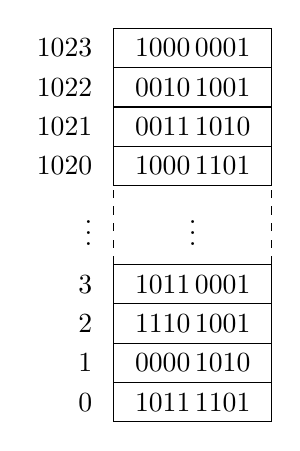
\begin{tikzpicture}
\pgfmathsetmacro{\kystep}{0.5}
\pgfmathsetmacro{\kxstep}{2}
\draw[](0,0)--++(0,4*\kystep) (0,6*\kystep)--++(0,4*\kystep)  (\kxstep,0)--++(0,4*\kystep)  (\kxstep,6*\kystep)--++(0,4*\kystep);
\draw[dashed](0,4*\kystep)--++(0,2*\kystep)  (\kxstep,4*\kystep)--++(0,2*\kystep);
\foreach \x in {0,1,2,3,4,6,7,8,9,10}{\draw(0,\x*\kystep)--++(\kxstep,0);}
\foreach \x/\a in {0/{1011\,1101},1/{0000\,1010},2/{1110\,1001},3/{1011\,0001}}{\draw(0.5*\kxstep,0.5*\kystep+\x*\kystep)node[]{$\a$};}
\foreach \x/\a in {6/{1000\,1101},7/{0011\,1010},8/{0010\,1001},9/{1000\,0001}}{\draw(0.5*\kxstep,0.5*\kystep+\x*\kystep)node[]{$\a$};}
\draw(0.5*\kxstep,5*\kystep)node[]{$\vdots$};
\draw(0,5*\kystep)node[left,xshift=-1ex]{$\vdots$};
\foreach \x/\a in {0/0,1/1,2/2,3/3,6/1020,7/1021,8/1022,9/1023}{\draw(0,0.5*\kystep+\x*\kystep)node[left,xshift=-1ex]{$\a$};}
\end{tikzpicture}
\caption{}
\end{subfigure}
\caption{حافظہ کی تصوراتی تصویر}
\label{شکل_حافظہ_تصوراتی_شکل}
\end{figure}

\ابتدا{مشق}
عارضی حافظہ \عددی{6116 }کے معلوماتی صفحات سے اس کی استعداد " کلو بائٹ " میں معلوم کریں۔
\انتہا{مشق}



\حصہ{ پختہ حافظہ}
پختہ حافظے سے مراد ا وہ حافظہ ہے جس میں مواد برقی طاقت کی عدم موجودگی میں بھی محفوظ رہتا ہو۔پختہ حافظہ کا بنیادی استعمال وہاں ہو گا جہاں مواد تبدیل نہ ہو۔

عارضی حافظے کی طرح پختہ حافظہ بھی مختلف لمبائی کے الفاظ پر مشتمل ہو گا۔لفظوں تک رسائی پتہ کے ذریعہ ہو گی؛ \عددی{n} بِٹ پتہ کے پختہ حافظہ میں \عددی{2^n} لفظ ہوں گے۔

بائٹ لمبائی چار لفظ پختہ حافظے کی اندرونی ساخت شکل  \حوالہ{شکل_حافظہ_چار_بائٹ_پختہ}  میں دکھائی گئی ہے جس کی بہتر صورت شکل  \حوالہ{شکل_حافظہ_پختہ_بہتر_صورت} پیش کرتی ہے ، جہاں چار داخلی جمع گیٹ کی صاف شکل استعمال کی گئی ہے۔مستعمل دو سے چار شناخت کار، پتہ کے دو بِٹ سے چار مقامات تک رسائی ممکن بناتا ہے۔یوں چار الفاظ تک رسائی ممکن ہو گی۔
\begin{figure}
\centering
\begin{tikzpicture}[
 kmemUnit/.style={draw, minimum height=0.75cm, minimum width=0.75cm,thick,
 label={[anchor=west]center:اکائی},
 }]
\pgfmathsetmacro{\ksepX}{1.00}
\pgfmathsetmacro{\ksepY}{1.25}
\pgfmathsetmacro{\kpin}{0.5}
\pgfmathsetmacro{\kpinA}{0.3}
\pgfmathsetmacro{\kpsep}{0.50}
\pgfmathsetmacro{\kul}{0.50}
\pgfmathsetmacro{\kmv}{0.15}
\pgfmathsetmacro{\kxdim}{2*\kul+1*\kpsep}
\pgfmathsetmacro{\kydim}{2*\kul+3*\kpsep}
\draw(-0*\ksepX,0)node[or port,number inputs=4,scale=0.8,rotate=-90](u0){} (u0.out)node[below]{$D_0$};
\draw(-1*\ksepX,0)node[or port,number inputs=4,scale=0.8,rotate=-90](u1){}(u1.out)node[below]{$D_1$};
\draw(-2*\ksepX,0)node[or port,number inputs=4,scale=0.8,rotate=-90](u2){}(u2.out)node[below]{$D_2$};
\draw(-3*\ksepX,0)node[or port,number inputs=4,scale=0.8,rotate=-90](u3){}(u3.out)node[below]{$D_3$};
\draw(-4*\ksepX,0)node[or port,number inputs=4,scale=0.8,rotate=-90](u4){}(u4.out)node[below]{$D_4$};
\draw(-5*\ksepX,0)node[or port,number inputs=4,scale=0.8,rotate=-90](u5){}(u5.out)node[below]{$D_5$};
\draw(-6*\ksepX,0)node[or port,number inputs=4,scale=0.8,rotate=-90](u6){}(u6.out)node[below]{$D_6$};
\draw(-7*\ksepX,0)node[or port,number inputs=4,scale=0.8,rotate=-90](u7){}(u7.out)node[below]{$D_7$};
\draw[thick](-8*\ksepX,\ksepY) rectangle ++(-\kxdim,\kydim);
\draw(-8*\ksepX,\ksepY+\kul)node[left]{$y_0$}coordinate(y0)--(y0 -| u0.in 1)--++(\kpinA,0)coordinate(kr)
node[right]{\RL{لفظ 0}};
\draw(-8*\ksepX,\ksepY+\kul+\kpsep)node[left]{$y_1$}coordinate(y1)--(y1 -| kr);
\draw(-8*\ksepX,\ksepY+\kul+2*\kpsep)node[left]{$y_2$}coordinate(y2)--(y2 -| kr);
\draw(-8*\ksepX,\ksepY+\kul+3*\kpsep)node[left]{$y_3$}coordinate(y3)--(y3 -| kr)node[right]{\RL{لفظ 3}};
\draw(-8*\ksepX-\kxdim,\ksepY+\kul+2*\kpsep)node[right]{$a_0$}--++(-\kpinA,0)node[left]{$A_0$};
\draw(-8*\ksepX-\kxdim,\ksepY+\kul+3*\kpsep)node[right]{$a_1$}--++(-\kpinA,0)node[left]{$A_1$};
\draw(-8*\ksepX-\kxdim,\ksepY+\kul)node[right]{$e$}--++(-\kpinA,0)node[left]{مجاز};
\draw(-8*\ksepX,\ksepY)++(-0.5*\kxdim,\kydim)node[above]{\RL{شناخت کار}};
\draw(u0.in 1)--(u0.in 1 |- y0)   (u0.in 2)--(u0.in 2 |- y1)  (u0.in 3)--(u0.in 3 |- y2)  (u0.in 4)--(u0.in 4 |- y3);
\draw(u1.in 1)--(u1.in 1 |- y0)   (u1.in 2)--(u1.in 2 |- y1)  (u1.in 3)--(u1.in 3 |- y2)  (u1.in 4)--(u1.in 4 |- y3);
\draw(u2.in 1)--(u2.in 1 |- y0)   (u2.in 2)--(u2.in 2 |- y1)  (u2.in 3)--(u2.in 3 |- y2)  (u2.in 4)--(u2.in 4 |- y3);
\draw(u3.in 1)--(u3.in 1 |- y0)   (u3.in 2)--(u3.in 2 |- y1)  (u3.in 3)--(u3.in 3 |- y2)  (u3.in 4)--(u3.in 4 |- y3);
\draw(u4.in 1)--(u4.in 1 |- y0)   (u4.in 2)--(u4.in 2 |- y1)  (u4.in 3)--(u4.in 3 |- y2)  (u4.in 4)--(u4.in 4 |- y3);
\draw(u5.in 1)--(u5.in 1 |- y0)   (u5.in 2)--(u5.in 2 |- y1)  (u5.in 3)--(u5.in 3 |- y2)  (u5.in 4)--(u5.in 4 |- y3);
\draw(u6.in 1)--(u6.in 1 |- y0)   (u6.in 2)--(u6.in 2 |- y1)  (u6.in 3)--(u6.in 3 |- y2)  (u6.in 4)--(u6.in 4 |- y3);
\draw(u7.in 1)--(u7.in 1 |- y0)   (u7.in 2)--(u7.in 2 |- y1)  (u7.in 3)--(u7.in 3 |- y2)  (u7.in 4)--(u7.in 4 |- y3);
\end{tikzpicture}
\caption{چار بائٹ پختہ حافظہ کی اندرونی ساخت}
\label{شکل_حافظہ_چار_بائٹ_پختہ}
\end{figure}
\begin{figure}
\centering
\begin{tikzpicture}[
 kmemUnit/.style={draw, minimum height=0.75cm, minimum width=0.75cm,thick,
 label={[anchor=west]center:اکائی},
 }]
\pgfmathsetmacro{\ksepX}{1.10}
\pgfmathsetmacro{\ksepY}{0.5}
\pgfmathsetmacro{\kpin}{0.5}
\pgfmathsetmacro{\kpinA}{0.3}
\pgfmathsetmacro{\kpsep}{0.50}
\pgfmathsetmacro{\kul}{0.50}
\pgfmathsetmacro{\kmv}{0.15}
\pgfmathsetmacro{\kxdim}{2*\kul+1*\kpsep}
\pgfmathsetmacro{\kydim}{2*\kul+3*\kpsep}
\kBusORdown[uu0]{-0*\ksepX}{0}
\kBusORdown[uu1]{-1*\ksepX}{0}
\kBusORdown[uu2]{-2*\ksepX}{0}
\kBusORdown[uu3]{-3*\ksepX}{0}
\kBusORdown[uu4]{-4*\ksepX}{0}
\kBusORdown[uu5]{-5*\ksepX}{0}
\kBusORdown[uu6]{-6*\ksepX}{0}
\kBusORdown[uu7]{-7*\ksepX}{0}
\draw(uu0out)--++(0,-\kpinA)node[below]{$D_0$};
\draw(uu1out)--++(0,-\kpinA)node[below]{$D_1$};
\draw(uu2out)--++(0,-\kpinA)node[below]{$D_2$};
\draw(uu3out)--++(0,-\kpinA)node[below]{$D_3$};
\draw(uu4out)--++(0,-\kpinA)node[below]{$D_4$};
\draw(uu5out)--++(0,-\kpinA)node[below]{$D_5$};
\draw(uu6out)--++(0,-\kpinA)node[below]{$D_6$};
\draw(uu7out)--++(0,-\kpinA)node[below]{$D_7$};
\draw[thick](-7*\ksepX-\kpin,\ksepY)coordinate(aa) rectangle ++(-\kxdim,\kydim)coordinate(tt);
\draw[thin](aa)++(0,\kul+0*\kpin)node[left]{$y_0$}coordinate(bb)--(bb -| uu0in)--++(\kpinA,0)coordinate(krt)node[right]{};
\draw(aa)++(0,\kul+1*\kpin)node[left]{$y_1$}coordinate(cc)--(cc -| krt);
\draw(aa)++(0,\kul+2*\kpin)node[left]{$y_2$}coordinate(dd)--(dd -| krt);
\draw(aa)++(0,\kul+3*\kpin)node[left]{$y_3$}coordinate(ee)--(ee -| krt);
\draw(aa)++(-0.5*\kxdim,\kydim)node[above]{\RL{شناخت کار}};
\draw(uu0in)--(uu0in |- tt);
\draw(uu1in)--(uu1in |- tt);
\draw(uu2in)--(uu2in |- tt);
\draw(uu3in)--(uu3in |- tt);
\draw(uu4in)--(uu4in |- tt);
\draw(uu5in)--(uu5in |- tt);
\draw(uu6in)--(uu6in |- tt);
\draw(uu7in)--(uu7in |- tt);
\draw(uu0in)++(-0.5*\kmv,\kpin)--++(\kmv,\kmv)node[right]{$4$}; 
\draw(uu1in)++(-0.5*\kmv,\kpin)--++(\kmv,\kmv)node[right]{$4$}; 
\draw(uu2in)++(-0.5*\kmv,\kpin)--++(\kmv,\kmv)node[right]{$4$}; 
\draw(uu3in)++(-0.5*\kmv,\kpin)--++(\kmv,\kmv)node[right]{$4$}; 
\draw(uu4in)++(-0.5*\kmv,\kpin)--++(\kmv,\kmv)node[right]{$4$}; 
\draw(uu5in)++(-0.5*\kmv,\kpin)--++(\kmv,\kmv)node[right]{$4$}; 
\draw(uu6in)++(-0.5*\kmv,\kpin)--++(\kmv,\kmv)node[right]{$4$}; 
\draw(uu7in)++(-0.5*\kmv,\kpin)--++(\kmv,\kmv)node[right]{$4$}; 
\draw[thin](aa)++(-\kxdim,\kul+0*\kpin)node[right]{$e$}--++(-\kpinA,0)node[left]{مجاز};
\draw[thin](aa)++(-\kxdim,\kul+2*\kpin)node[right]{$a_0$}--++(-\kpinA,0)node[left]{$A_0$};
\draw[thin](aa)++(-\kxdim,\kul+3*\kpin)node[right]{$a_1$}--++(-\kpinA,0)node[left]{$A_1$};
\end{tikzpicture}
\caption{چار بائٹ پختہ حافظہ کی اندرونی ساخت}
\label{شکل_حافظہ_پختہ_بہتر_صورت}
\end{figure}

شکل  \حوالہ{شکل_حافظہ_چار_بائٹ_پختہ}  میں بالکل نیا غیر استعمال شدہ پختہ حافظہ دکھایا گیا ہے۔پتہ \عددی{00_2} کی صورت میں دو سے چار شناخت کار \عددی{y_0} بلند کر کے لفظ \عددی{0} چنے گا۔ تمام جمع گیٹ بلند ہوں گے اور \عددی{D} پر \عددی{11111111_2} خارج ہو گا۔ پتہ \عددی{01_2} لفظ \عددی{1} چنے گا اور \عددی{D} پر \عددی{11111111_2} خارج ہو گا۔آپ تسلی کر لیں کہ چاروں پتہ پر یہی مواد ملتا ہے۔کسی بھی نئے غیر استعمال شدہ پختہ حافظے کے ہر لفظ کے تمام بِٹ بلند \عددی{(1)} ہوں گے۔


آپ نے دیکھا کہ بلند \عددی{y_0} کی صورت میں تمام جمع گیٹ کو یہی بلند اشارہ ملتا ہے اور یوں تمام جمع گیٹ کے مخارج بلند ہو ں گے۔جمع گیٹ سے \عددی{y_0} کا جوڑ منقطع کرنے سے \عددی{y_0} جمع گیٹ تک نہیں پہنچے گا۔شکل  \حوالہ{شکل_حافظہ_پختہ_لکھائی}  میں دائیں چار جمع  گیٹ \عددی{y_0} سے منقطع ہیں لہٰذا \عددی{y_0} بلند کر کے لفظ \عددی{0} پڑھنے سے \عددی{D} پر \عددی{11110000_2} ملتا ہے۔یہاں ایک بات ذہن نشین کریں :ایسے اشکال میں جمع گیٹ کا منقطع مداخل جمع گیٹ کے مخارج پر اثر انداز نہیں ہو گا۔
\begin{figure}
\centering
\begin{tikzpicture}[
 kmemUnit/.style={draw, minimum height=0.75cm, minimum width=0.75cm,thick,
 label={[anchor=west]center:اکائی},
 }]
\pgfmathsetmacro{\ksepX}{1.00}
\pgfmathsetmacro{\ksepY}{1.25}
\pgfmathsetmacro{\kpin}{0.5}
\pgfmathsetmacro{\kpinA}{0.3}
\pgfmathsetmacro{\kpsep}{0.50}
\pgfmathsetmacro{\kul}{0.50}
\pgfmathsetmacro{\kmv}{0.15}
\pgfmathsetmacro{\kxdim}{2*\kul+1*\kpsep}
\pgfmathsetmacro{\kydim}{2*\kul+3*\kpsep}
\draw(-0*\ksepX,0)node[or port,number inputs=4,scale=0.8,rotate=-90](u0){} (u0.out)node[below]{$D_0$};
\draw(-1*\ksepX,0)node[or port,number inputs=4,scale=0.8,rotate=-90](u1){}(u1.out)node[below]{$D_1$};
\draw(-2*\ksepX,0)node[or port,number inputs=4,scale=0.8,rotate=-90](u2){}(u2.out)node[below]{$D_2$};
\draw(-3*\ksepX,0)node[or port,number inputs=4,scale=0.8,rotate=-90](u3){}(u3.out)node[below]{$D_3$};
\draw(-4*\ksepX,0)node[or port,number inputs=4,scale=0.8,rotate=-90](u4){}(u4.out)node[below]{$D_4$};
\draw(-5*\ksepX,0)node[or port,number inputs=4,scale=0.8,rotate=-90](u5){}(u5.out)node[below]{$D_5$};
\draw(-6*\ksepX,0)node[or port,number inputs=4,scale=0.8,rotate=-90](u6){}(u6.out)node[below]{$D_6$};
\draw(-7*\ksepX,0)node[or port,number inputs=4,scale=0.8,rotate=-90](u7){}(u7.out)node[below]{$D_7$};
\draw[thick](-8*\ksepX,\ksepY) rectangle ++(-\kxdim,\kydim);
\draw(-8*\ksepX,\ksepY+\kul)node[left]{$y_0$}coordinate(y0)--(y0 -| u0.in 1)--++(\kpinA,0)coordinate(kr)
node[right]{\RL{لفظ 0}};
\draw(-8*\ksepX,\ksepY+\kul+\kpsep)node[left]{$y_1$}coordinate(y1)--(y1 -| kr);
\draw(-8*\ksepX,\ksepY+\kul+2*\kpsep)node[left]{$y_2$}coordinate(y2)--(y2 -| kr);
\draw(-8*\ksepX,\ksepY+\kul+3*\kpsep)node[left]{$y_3$}coordinate(y3)--(y3 -| kr)node[right]{\RL{لفظ 3}};
\draw(-8*\ksepX-\kxdim,\ksepY+\kul+2*\kpsep)node[right]{$a_0$}--++(-\kpinA,0)node[left]{$A_0$};
\draw(-8*\ksepX-\kxdim,\ksepY+\kul+3*\kpsep)node[right]{$a_1$}--++(-\kpinA,0)node[left]{$A_1$};
\draw(-8*\ksepX-\kxdim,\ksepY+\kul)node[right]{$e$}--++(-\kpinA,0)node[left]{مجاز};
\draw(-8*\ksepX,\ksepY)++(-0.5*\kxdim,\kydim)node[above]{\RL{شناخت کار}};
\draw(u0.in 1)--++(0,0.5*\kpin)   (u0.in 2)--(u0.in 2 |- y1)  (u0.in 3)--(u0.in 3 |- y2)  (u0.in 4)--(u0.in 4 |- y3);
\draw(u1.in 1)--++(0,0.5*\kpin)    (u1.in 2)--(u1.in 2 |- y1)  (u1.in 3)--(u1.in 3 |- y2)  (u1.in 4)--(u1.in 4 |- y3);
\draw(u2.in 1)--++(0,0.5*\kpin)    (u2.in 2)--(u2.in 2 |- y1)  (u2.in 3)--(u2.in 3 |- y2)  (u2.in 4)--(u2.in 4 |- y3);
\draw(u3.in 1)--++(0,0.5*\kpin)    (u3.in 2)--(u3.in 2 |- y1)  (u3.in 3)--(u3.in 3 |- y2)  (u3.in 4)--(u3.in 4 |- y3);
\draw(u4.in 1)--(u4.in 1 |- y0)   (u4.in 2)--(u4.in 2 |- y1)  (u4.in 3)--(u4.in 3 |- y2)  (u4.in 4)--(u4.in 4 |- y3);
\draw(u5.in 1)--(u5.in 1 |- y0)   (u5.in 2)--(u5.in 2 |- y1)  (u5.in 3)--(u5.in 3 |- y2)  (u5.in 4)--(u5.in 4 |- y3);
\draw(u6.in 1)--(u6.in 1 |- y0)   (u6.in 2)--(u6.in 2 |- y1)  (u6.in 3)--(u6.in 3 |- y2)  (u6.in 4)--(u6.in 4 |- y3);
\draw(u7.in 1)--(u7.in 1 |- y0)   (u7.in 2)--(u7.in 2 |- y1)  (u7.in 3)--(u7.in 3 |- y2)  (u7.in 4)--(u7.in 4 |- y3);
\end{tikzpicture}
\caption{پختہ حافظہ میں لکھائی}
\label{شکل_حافظہ_پختہ_لکھائی}
\end{figure}

امید کی جاتی ہے آپ پختہ حافظہ میں لکھائی کا عمل بخوبی سمجھ گئے ہوں گے۔پختہ حافظے میں جوڑوں کو توڑ کر مواد لکھا جاتا ہے۔اس قسم حافظہ میں ہر جوڑ دراصل ایک\اصطلاح{ برقی فتیلہ }\فرہنگ{فتیلہ}\حاشیہب{electric fuse}\فرہنگ{fuse} (فیوز ) ہو تا ہے ۔ فتیلے کی استعداد سے زیادہ برقی رو فتیلے سے گزار کر اسے پگھلا کر جوڑ منقطع کیا جاتا ہے۔


حافظہ میں لکھا مواد شکل \حوالہ{شکل_حافظہ_تصوراتی_شکل} کی طرح جدول میں لکھا جاتا ہے۔اس جدول میں باری باری ایک لفظ کو دیکھتے ہوئے جس بِٹ کے مقام پر \عددی{0} ہو، حافظہ کے اندر اس لفظ کے اس بِٹ کا جوڑ تباہ کیا جاتا ہے۔

\begin{figure}
\centering
\begin{subfigure}{1\textwidth}
\centering
\begin{tikzpicture}[
 kmemUnit/.style={draw, minimum height=0.75cm, minimum width=0.75cm,thick,
 label={[anchor=west]center:اکائی},
 }]
\pgfmathsetmacro{\ksepX}{1.10}
\pgfmathsetmacro{\ksepY}{0.5}
\pgfmathsetmacro{\kpin}{0.5}
\pgfmathsetmacro{\kpinA}{0.3}
\pgfmathsetmacro{\kpsep}{0.50}
\pgfmathsetmacro{\kul}{0.50}
\pgfmathsetmacro{\kmv}{0.15}
\pgfmathsetmacro{\kxdim}{2*\kul+1*\kpsep}
\pgfmathsetmacro{\kydim}{2*\kul+3*\kpsep}
\kBusORdown[uu0]{-0*\ksepX}{0}
\kBusORdown[uu1]{-1*\ksepX}{0}
\kBusORdown[uu2]{-2*\ksepX}{0}
\kBusORdown[uu3]{-3*\ksepX}{0}
\kBusORdown[uu4]{-4*\ksepX}{0}
\kBusORdown[uu5]{-5*\ksepX}{0}
\kBusORdown[uu6]{-6*\ksepX}{0}
\kBusORdown[uu7]{-7*\ksepX}{0}
\draw(uu0out)--++(0,-\kpinA)node[below]{$D_0$};
\draw(uu1out)--++(0,-\kpinA)node[below]{$D_1$};
\draw(uu2out)--++(0,-\kpinA)node[below]{$D_2$};
\draw(uu3out)--++(0,-\kpinA)node[below]{$D_3$};
\draw(uu4out)--++(0,-\kpinA)node[below]{$D_4$};
\draw(uu5out)--++(0,-\kpinA)node[below]{$D_5$};
\draw(uu6out)--++(0,-\kpinA)node[below]{$D_6$};
\draw(uu7out)--++(0,-\kpinA)node[below]{$D_7$};
\draw[thick](-7*\ksepX-\kpin,\ksepY)coordinate(aa) rectangle ++(-\kxdim,\kydim)coordinate(tt);
\draw[thin](aa)++(0,\kul+0*\kpin)node[left]{$y_0$}coordinate(bb)--(bb -| uu0in)--++(\kpinA,0)coordinate(krt)node[right]{};
\draw(aa)++(0,\kul+1*\kpin)node[left]{$y_1$}coordinate(cc)--(cc -| krt);
\draw(aa)++(0,\kul+2*\kpin)node[left]{$y_2$}coordinate(dd)--(dd -| krt);
\draw(aa)++(0,\kul+3*\kpin)node[left]{$y_3$}coordinate(ee)--(ee -| krt);
\draw(aa)++(-0.5*\kxdim,\kydim)node[above]{\RL{شناخت کار}};
\draw(uu0in)--(uu0in |- tt);
\draw(uu1in)--(uu1in |- tt);
\draw(uu2in)--(uu2in |- tt);
\draw(uu3in)--(uu3in |- tt);
\draw(uu4in)--(uu4in |- tt);
\draw(uu5in)--(uu5in |- tt);
\draw(uu6in)--(uu6in |- tt);
\draw(uu7in)--(uu7in |- tt);
\draw[thin](aa)++(-\kxdim,\kul+0*\kpin)node[right]{$e$}--++(-\kpinA,0)node[left]{مجاز};
\draw[thin](aa)++(-\kxdim,\kul+2*\kpin)node[right]{$a_0$}--++(-\kpinA,0)node[left]{$A_0$};
\draw[thin](aa)++(-\kxdim,\kul+3*\kpin)node[right]{$a_1$}--++(-\kpinA,0)node[left]{$A_1$};
\path(uu0in)--(uu0in |- cc)coordinate(aaaa);
\draw(aaaa)++(-0.5*\kmv,-0.5*\kmv)--++(\kmv,\kmv)  (aaaa)++(-0.5*\kmv,0.5*\kmv)--++(\kmv,-\kmv);
\path(uu0in)--(uu0in |- dd)coordinate(aaaa);
\draw(aaaa)++(-0.5*\kmv,-0.5*\kmv)--++(\kmv,\kmv)  (aaaa)++(-0.5*\kmv,0.5*\kmv)--++(\kmv,-\kmv);
\path(uu1in)--(uu1in |- bb)coordinate(aaaa);
\draw(aaaa)++(-0.5*\kmv,-0.5*\kmv)--++(\kmv,\kmv)  (aaaa)++(-0.5*\kmv,0.5*\kmv)--++(\kmv,-\kmv);
\path(uu2in)--(uu2in |- cc)coordinate(aaaa);
\draw(aaaa)++(-0.5*\kmv,-0.5*\kmv)--++(\kmv,\kmv)  (aaaa)++(-0.5*\kmv,0.5*\kmv)--++(\kmv,-\kmv);
\path(uu2in)--(uu2in |- ee)coordinate(aaaa);
\draw(aaaa)++(-0.5*\kmv,-0.5*\kmv)--++(\kmv,\kmv)  (aaaa)++(-0.5*\kmv,0.5*\kmv)--++(\kmv,-\kmv);
\path(uu3in)--(uu3in |- dd)coordinate(aaaa);
\draw(aaaa)++(-0.5*\kmv,-0.5*\kmv)--++(\kmv,\kmv)  (aaaa)++(-0.5*\kmv,0.5*\kmv)--++(\kmv,-\kmv);
\path(uu3in)--(uu3in |- ee)coordinate(aaaa);
\draw(aaaa)++(-0.5*\kmv,-0.5*\kmv)--++(\kmv,\kmv)  (aaaa)++(-0.5*\kmv,0.5*\kmv)--++(\kmv,-\kmv);
\path(uu4in)--(uu4in |- bb)coordinate(aaaa);
\draw(aaaa)++(-0.5*\kmv,-0.5*\kmv)--++(\kmv,\kmv)  (aaaa)++(-0.5*\kmv,0.5*\kmv)--++(\kmv,-\kmv);
\path(uu5in)--(uu5in |- bb)coordinate(aaaa);
\draw(aaaa)++(-0.5*\kmv,-0.5*\kmv)--++(\kmv,\kmv)  (aaaa)++(-0.5*\kmv,0.5*\kmv)--++(\kmv,-\kmv);
\path(uu5in)--(uu5in |- cc)coordinate(aaaa);
\draw(aaaa)++(-0.5*\kmv,-0.5*\kmv)--++(\kmv,\kmv)  (aaaa)++(-0.5*\kmv,0.5*\kmv)--++(\kmv,-\kmv);
\path(uu5in)--(uu5in |- dd)coordinate(aaaa);
\draw(aaaa)++(-0.5*\kmv,-0.5*\kmv)--++(\kmv,\kmv)  (aaaa)++(-0.5*\kmv,0.5*\kmv)--++(\kmv,-\kmv);
\path(uu6in)--(uu6in |- cc)coordinate(aaaa);
\draw(aaaa)++(-0.5*\kmv,-0.5*\kmv)--++(\kmv,\kmv)  (aaaa)++(-0.5*\kmv,0.5*\kmv)--++(\kmv,-\kmv);
\path(uu6in)--(uu6in |- dd)coordinate(aaaa);
\draw(aaaa)++(-0.5*\kmv,-0.5*\kmv)--++(\kmv,\kmv)  (aaaa)++(-0.5*\kmv,0.5*\kmv)--++(\kmv,-\kmv);
\path(uu7in)--(uu7in |- bb)coordinate(aaaa);
\draw(aaaa)++(-0.5*\kmv,-0.5*\kmv)--++(\kmv,\kmv)  (aaaa)++(-0.5*\kmv,0.5*\kmv)--++(\kmv,-\kmv);
\path(uu7in)--(uu7in |- ee)coordinate(aaaa);
\draw(aaaa)++(-0.5*\kmv,-0.5*\kmv)--++(\kmv,\kmv)  (aaaa)++(-0.5*\kmv,0.5*\kmv)--++(\kmv,-\kmv);
\end{tikzpicture}
\caption{}
\end{subfigure}
\begin{subfigure}{1\textwidth}
\centering
\begin{otherlanguage}{english}
\begin{tabular}{C|C}
\toprule
\text{\RL{پتہ}}&\text{\RL{مواد}}\\
\midrule
00&1011\,0010\\
01&0110\,0101\\
10&0110\,1001\\
11&1000\,1100\\
\bottomrule
\end{tabular}
\end{otherlanguage}
\caption{}
\end{subfigure}
\caption{پختہ حافظہ  میں لکھا گیا  مواد}
\label{شکل_حافظہ_پختہ_لکھا_مواد}
\end{figure}
 شکل  \حوالہ{شکل_حافظہ_پختہ_لکھا_مواد}-ا   میں غیر تباہ شدہ جوڑ صلیبی نشان \عددی{(\times)} سے ظاہر کیے  گئے ہیں۔ اس حافظہ میں لکھا مواد شکل-ب میں پیش ہے۔

اب تک چار لفظ حافظہ پر بات کی گئی جس کی وجہ سے \عددی{4} داخلی جمع گیٹ استعمال کیے گئے۔ایک لفظ \عددی{8} بِٹ ہونے کی وجہ سے کل \عددی{8} جمع گیٹ استعمال کیے گئے۔یوں ان حافظوں میں کل \عددی{8\times 4} یعنی بتیس \عددی{(32)} جوڑ یا فتیلے ہوں گے۔ آپ دیکھ سکتے ہیں کہ \عددی{n} بِٹ پتے کے حافظے میں \عددی{2^n} لفظ ہوں گے لہٰذا ایسے حافظے میں \عددی{2^n} داخلی جمع گیٹ ہوں گے۔اگر حافظے کا ایک لفظ \عددی{m} بِٹ ہو تب جمع گیٹوں کی تعداد \عددی{m} ہو گی۔یوں حافظے میں جوڑوں کی تعداد \عددی{m\times 2^n} ہو گی۔

\اصطلاح{شعاع مٹتا پختہ حافظہ } میں بار بار لکھائی ممکن ہے۔ان میں جوڑ، برقی فتیلہ سے نہیں بنائے جاتے بلکہ ان جوڑ کو ایک\اصطلاح{ سوئچ }\فرہنگ{سوئچ}\حاشیہب{switch}\فرہنگ{switch} تصور کریں جنہیں مخصوص طریقے سے برقی طاقت کے ذریعہ منقطع کیا جا تا ہے۔منقطع جوڑوں کو دوبارہ جوڑنے کی خاطر حافظے کو شعاع میں کچھ دیر رکھا جاتا ہے۔

جدید\اصطلاح{ برق مٹتا پختہ حافظوں } میں بار بار لکھائی ممکن ہے۔ان حافظوں میں لکھائی برقی دباو سے کی جاتی ہے اور اسے صاف بھی برقی دباو سے کیا جاتا ہے۔

پختہ حافظہ میں لکھائی \اصطلاح{ مخلوط ادوار برنامہ نویس }\فرہنگ{مخلوط دور!برنامہ نویس}\حاشیہب{IC programmer}\فرہنگ{IC!programmer} کی مدد سے کی جاتی ہے۔
	

\حصہ{حافظہ کی استعداد بڑھانے کی ترکیب}
عارضی حافظوں ( کے مخلوط ادوار ) کے قابو مداخل عموماً \عددی{\overline{\text{\RL{بیدار}}}}، \عددی{\overline{\text{\RL{مجاز}}}}اور \عددی{\overline{\text{\RL{لکھ}}}/\text{\RL{پڑھ}}} جبکہ پختہ حافظوں کے \عددی{\overline{\text{\RL{بیدار}}}} اور \عددی{\overline{\text{\RL{مجاز}}}} ہوں گے۔اس حصے میں ہم تصور کرتے ہیں کہ حافظوں کے قابو اشارات صرف \عددی{\overline{\text{\RL{بیدار}}}} اور \عددی{\overline{\text{\RL{لکھ}}}/\text{\RL{پڑھ}}} ہیں جنہیں استعمال کرتے ہوئے ایک سے زیادہ حافظے آپس میں جوڑنا دکھایا جائے گا۔حقیقت میں عموماً \عددی{\overline{\text{\RL{بیدار}}}} کے علاوہ تمام حافظوں کے ایک جیسے قابو مداخل ایک ساتھ جوڑے جاتے ہیں۔یوں تمام حافظوں کے \عددی{\overline{\text{\RL{مجاز}}}} مداخل اکٹھے جوڑے جائیں گے اور اسی طرح تمام کے \عددی{\overline{\text{\RL{لکھ}}}/\text{\RL{پڑھ}}} ایک ساتھ جوڑے جائیں گے۔

\جزوحصہ{دو عدد \عددی{4\times 4} حافظے سلسلہ وار جوڑ کر ایک عدد \عددی{8\times 4} حافظہ کا حصول}
کبھی کبھار درکار استعداد کا حافظہ میسر نہیں ہو گا۔ایسی صورت میں ایک سے زیادہ حافظے اکٹھے جوڑ کر درکار بائٹ ذخیرہ کرنا ممکن بنایا جاتا ہے۔شکل \حوالہ{شکل_حافظہ_بڑے_حافظہ_کا_حصول}-ا میں \عددی{4\times 4} کے دو حافظے جوڑ کر دگنی استعداد کا \عددی{8\times 4} حافظہ  (شکل-ب)حاصل کیا گیا۔چھوٹے حافظوں کو حافظہ 0 اور حافظہ 1 کہا گیا ہے۔ شکل-ا میں ایک جیسے پتہ بِٹ ساتھ ساتھ جوڑے گئے ہیں یعنی حافظہ 0 کا \عددی{A_0} حافظہ 1 کے \عددی{A_0} سے جوڑا گیا ہے، اور حافظہ 0 کا \عددی{A_1} حافظہ 1 کے \عددی{A_1} سے جوڑا گیا ہے۔اسی طرح ایک جیسے مواد بِٹ ساتھ ساتھ جوڑے گئے ہیں یعنی حافظہ 0 کے \عددی{D_0}، \عددی{D_1}، \عددی{D_2} اور \عددی{D_3} بالترتیب حافظہ 1 کے \عددی{D_0}، \عددی{D_1}، \عددی{D_2} اور \عددی{D_3} سے جوڑے گئے ہیں۔البتہ حافظہ 0 کا \عددی{\overline{\text{\RL{بیدار}}}} مداخل (جسے \عددی{\overline{\text{\RL{بیدار0}}}}کہا گیا ہے) سیدھا \عددی{A_2} کے ساتھ ملایا گیا ہے جبکہ حافظہ 1 کا \عددی{\overline{\text{\RL{بیدار}}}} مداخل (جسے \عددی{\overline{\text{\RL{بیدار1}}}} کہا گیا ہے) نفی گیٹ کے ذریعہ \عددی{A_2} سے جوڑا گیا ہے۔ حافظہ 0، حافظہ 1 ، اور نفی گیٹ  کو  ہم ایک بڑا حافظہ تصور کر سکتے ہیں جس کی علامت شکل-ب میں پیش ہے۔

\begin{figure}
\centering
\begin{subfigure}{1\textwidth}
\centering
\begin{tikzpicture}
\pgfmathsetmacro{\ksepX}{1.10}
\pgfmathsetmacro{\ksepY}{4}
\pgfmathsetmacro{\kpin}{0.5}
\pgfmathsetmacro{\kpinA}{0.3}
\pgfmathsetmacro{\kpsep}{0.50}
\pgfmathsetmacro{\kul}{0.50}
\pgfmathsetmacro{\kmv}{0.15}
\pgfmathsetmacro{\kxdim}{2*\kul+2*\kpsep}
\pgfmathsetmacro{\kydim}{2*\kul+4*\kpsep}
\draw[thick](0,0) rectangle++(\kxdim,\kydim);
\draw[thick](0,\ksepY) rectangle++(\kxdim,\kydim);
\draw(0.5*\kxdim,\kydim)node[above]{\text{\RL{\عددی{4\times 4}  حافظہ 0}}};
\draw(0.5*\kxdim,\ksepY+\kydim)node[above]{\text{\RL{\عددی{4\times 4}  حافظہ 1}}};
\draw(0,\ksepY)++(\kxdim,\kul+1*\kpsep)coordinate(aa)node[left]{$I\!/\!O_0$}--++(5*\kpin,0)node[right]{$D_0$};
\draw(0,\ksepY)++(\kxdim,\kul+2*\kpsep)coordinate(bb)node[left]{$I\!/\!O_1$}--++(5*\kpin,0)node[right]{$D_1$};
\draw(0,\ksepY)++(\kxdim,\kul+3*\kpsep)coordinate(cc)node[left]{$I\!/\!O_2$}--++(5*\kpin,0)node[right]{$D_2$};
\draw(0,\ksepY)++(\kxdim,\kul+4*\kpsep)coordinate(dd)node[left]{$I\!/\!O_3$}--++(5*\kpin,0)node[right]{$D_3$};
\draw(\kxdim,\kul+4*\kpsep)node[left]{$I\!/\!O_3$}--++(\kpin,0)coordinate(ee)--(ee |- dd);
\draw(\kxdim,\kul+3*\kpsep)node[left]{$I\!/\!O_2$}--++(2*\kpin,0)coordinate(ff)--(ff |- cc);
\draw(\kxdim,\kul+2*\kpsep)node[left]{$I\!/\!O_1$}--++(3*\kpin,0)coordinate(gg)--(gg |- bb);
\draw(\kxdim,\kul+1*\kpsep)node[left]{$I\!/\!O_0$}--++(4*\kpin,0)coordinate(hh)--(hh |- aa);
\draw(0,\ksepY+\kul)node[right]{$\overline{\text{\RL{بیدار1}}}$}--++(-4*\kpin,0)node[not port,scale=1,anchor=out](u0){};
\draw(0,\ksepY+\kul)++(-0.05,0)node[ocirc]{};
\draw(u0.in)--++(-\kpin,0)coordinate(klft)node[left]{$A_2$};
\draw(0,\kul)node[right]{$\overline{\text{\RL{بیدار0}}}$}-|(u0.in);
\draw(0,\kul)++(-0.05,0)node[ocirc]{};
\draw(0,\kul+\kpin)coordinate(rd)--(rd -| klft)node[left]{$\overline{\text{لکھ}}/\text{پرھ}$};
\draw(0,\kul+\kpin)node[right]{$\overline{\text{لکھ}}$}++(-0.05,0)node[ocirc]{};
\draw(0,\kul+3*\kpin)node[right]{$A_0$}coordinate(ka0)--(ka0 -| klft)node[left]{$A_0$};
\draw(0,\kul+4*\kpin)node[right]{$A_1$}coordinate(ka1)--(ka1 -| klft)node[left]{$A_1$};
\draw(0,\ksepY+\kul+1*\kpin)node[right]{$\overline{\text{لکھ}}$}--++(-\kpin,0)coordinate(kka)--(kka |- rd);
\draw(0,\ksepY+\kul+1*\kpin)++(-0.05,0)node[ocirc]{};
\draw(0,\ksepY+\kul+3*\kpin)node[right]{$A_0$}--++(-2*\kpin,0)coordinate(kka0)--(kka0|- ka0);
\draw(0,\ksepY+\kul+4*\kpin)node[right]{$A_1$}--++(-3*\kpin,0)coordinate(kka1)--(kka1|- ka1);
\end{tikzpicture}
\caption{}
\end{subfigure}
\begin{subfigure}{1\textwidth}
\centering
\begin{tikzpicture}
\pgfmathsetmacro{\ksepX}{1.10}
\pgfmathsetmacro{\ksepY}{4}
\pgfmathsetmacro{\kpin}{0.5}
\pgfmathsetmacro{\kpinA}{0.3}
\pgfmathsetmacro{\kpsep}{0.50}
\pgfmathsetmacro{\kul}{0.50}
\pgfmathsetmacro{\kmv}{0.15}
\pgfmathsetmacro{\kxdim}{2*\kul+2*\kpsep}
\pgfmathsetmacro{\kydim}{2*\kul+4*\kpsep}
\draw[thick](0,0) rectangle++(\kxdim,\kydim);
\draw(0.5*\kxdim,\kydim)node[above]{\text{\RL{\عددی{8\times 4}  حافظہ}}};
\foreach \x/\a/\b in {0/{A_0}/{A_0},1/{A_1}/{A_1},2/{A_2}/{A_2}}{\draw(0,\kul+2*\kpsep+\x*\kpsep)node[right]{$\a$}--++(-\kpin,0)node[left]{$\b$};}
\foreach \x/\a/\b in {0/{I\!/\!O_0}/D_0,1/{I\!/\!O_1}/D_1,2/{I\!/\!O_2}/D_2,3/{I\!/\!O_3}/D_3}{\draw(\kxdim,\kul+\kpin+\x*\kpsep)node[left]{$\a$}--++(\kpin,0)node[right]{$\b$};}
\draw(0,\kul)node[right]{$\overline{\text{لکھ}}$}--++(-\kpin,0)node[left]{$\overline{\text{لکھ}}/\text{پڑھ}$};
\draw(0,\kul)++(-0.05,0)node[ocirc]{};
\end{tikzpicture}
\caption{}
\end{subfigure}
\caption{دو حافظے جوڑ کر بڑے حافظے کا حصول}
\label{شکل_حافظہ_بڑے_حافظہ_کا_حصول}
\end{figure}


شکل  \حوالہ{شکل_حافظہ_کل_میں_چھوٹے_کا_مقام}-ا میں تین پتہ بِٹ کی تمام  ترتیب دی گئی ہیں۔ (شکل \حوالہ{شکل_حافظہ_پختہ_لکھا_مواد}  دیکھتے ہوئے آگے پڑھیں۔) پست \عددی{A_2} سے مراد پست \عددی{\overline{\text{\RL{بیدار0}}}} اور بلند \عددی{\overline{\text{\RL{بیدار1}}}} ہوگا جس سے حافظہ 0 جاگ اٹھتا ہے اور حافظہ 1 نڈھال رہتا ہے۔اسی طرح بلند \عددی{A_2} سے \عددی{\overline{\text{\RL{بیدار0}}}} بلند اور \عددی{\overline{\text{\RL{بیدار1}}}} پست ہو گا جس سے حافظہ 0 نڈھال اور حافظہ 1 جاگ اٹھے گا ۔
\begin{figure}
\centering
\begin{subfigure}{1\textwidth}
\centering
\begin{tikzpicture}
\pgfmathsetmacro{\kystep}{0.5}
\pgfmathsetmacro{\kxstep}{1}
\foreach \x/\a in {0/1,1/1,2/1,3/1,4/0,5/0,6/0,7/0,8/{A_2}}{\draw(0,\x*\kystep)node[]{$\a$};}
\foreach \x/\a in {0/1,1/1,2/0,3/0,4/1,5/1,6/0,7/0,8/{A_1}}{\draw(\kxstep,\x*\kystep)node[]{$\a$};}
\foreach \x/\a in {0/1,1/0,2/1,3/0,4/1,5/0,6/1,7/0,8/{A_0}}{\draw(2*\kxstep,\x*\kystep)node[]{$\a$};}
\draw(-0.5*\kxstep,7.5*\kystep)--++(3*\kxstep,0);
\draw[dashed](0,5.5*\kystep) circle (0.5 and 1.9*\kystep);
\draw[](-0.5,5.5*\kystep) to [out=180,in=-45]++(-2,0.25)node[above]{\RL{حافظہ \عددی{0} بیدار ہے}};
\draw[dashed](0,1.5*\kystep) circle (0.5 and 1.9*\kystep);
\draw[](-0.5,1.5*\kystep) to [out=180,in=45]++(-2,-0.25)node[below]{\RL{حافظہ \عددی{1} بیدار ہے}};
\draw[dashed](0.75*\kxstep,6.5*\kystep) rectangle ++(1.5*\kxstep,0.9*\kystep);
\draw[] (0.75*\kxstep,6.5*\kystep) ++(1.5*\kxstep,0.45*\kystep) to [out=0,in=-150]++(2,0.25)node[right]{\RL{حافظہ \عددی{0} کا مقام \عددی{0}}};
\draw[dashed](0.75*\kxstep,2.5*\kystep) rectangle ++(1.5*\kxstep,0.9*\kystep);
\draw[] (0.75*\kxstep,2.5*\kystep) ++(1.5*\kxstep,0.45*\kystep) to [out=0,in=-150]++(2,0.25)node[right]{\RL{حافظہ \عددی{1} کا مقام \عددی{0}}};
\end{tikzpicture}
\caption{}
\end{subfigure}
\begin{subfigure}{1\textwidth}
\centering
\begin{tikzpicture}
\pgfmathsetmacro{\kystep}{0.5}
\pgfmathsetmacro{\kxstep}{1.25}
\pgfmathsetmacro{\ksepX}{4}
\pgfmathsetmacro{\ksepY}{0.25}
\draw[](0,0)--++(0,8*\kystep)  (\kxstep,0)--++(0,8*\kystep);
\foreach \x in {0,1,...,8}{\draw(0,\x*\kystep)--++(\kxstep,0);}
\foreach \x in {0,1,...,7}{\draw(0.5*\kxstep,0.5*\kystep+\x*\kystep)node[]{\RL{مقام \, \x}};}
\draw(0.5*\kxstep,0)node[below]{$8\times 4$};
\draw[](-\ksepX,-\ksepY)--++(0,4*\kystep)  (-\ksepX+\kxstep,-\ksepY)--++(0,4*\kystep);
\foreach \x in {0,1,...,4}{\draw(-\ksepX,-\ksepY+\x*\kystep)--++(\kxstep,0);}
\foreach \x in {0,1,...,3}{\draw(-\ksepX+0.5*\kxstep,-\ksepY+0.5*\kystep+\x*\kystep)node[]{\RL{مقام \, \x}};}
\draw[](-\ksepX,\ksepY+4*\kystep)--++(0,4*\kystep)  (-\ksepX+\kxstep,\ksepY+4*\kystep)--++(0,4*\kystep);
\foreach \x in {0,1,...,4}{\draw(-\ksepX,\ksepY+\x*\kystep+4*\kystep)--++(\kxstep,0);}
\foreach \x in {0,1,...,3}{\draw(-\ksepX+0.5*\kxstep,\ksepY+0.5*\kystep+\x*\kystep+4*\kystep)node[]{\RL{مقام \, \x}};}
\draw[decorate,decoration={brace,amplitude=10pt, raise=2pt}](0,0.1)--++(0,4*\kystep-0.2);
\draw[decorate,decoration={brace,amplitude=10pt, raise=2pt}](0,4*\kystep+0.1)--(0,8*\kystep-0.1);
\draw[decorate,decoration={brace,amplitude=10pt, raise=2pt,mirror}](-\ksepX+\kxstep,-\ksepY+0.1)--++(0,4*\kystep-0.2);
\draw[decorate,decoration={brace,amplitude=10pt, raise=2pt,mirror}](-\ksepX+\kxstep,4*\kystep+\ksepY+0.1)--++(0,4*\kystep-0.2);
\draw[-stealth] (-\ksepX+\kxstep+0.5,-\ksepY+2*\kystep) to [out=0,in=180] (-0.5,2*\kystep);
\draw[-stealth] (-\ksepX+\kxstep+0.5,\ksepY+6*\kystep) to [out=0,in=180] (-0.5,6*\kystep);
\draw(-\ksepX,-\ksepY+2*\kystep)node[left]{\RL{\عددی{4\times 4} حافظہ 0}};
\draw(-\ksepX,\ksepY+6*\kystep)node[left]{\RL{\عددی{4\times 4} حافظہ 1}};
\end{tikzpicture}
\caption{}
\end{subfigure}
\caption{کل حافظہ میں چھوٹے حافظوں کا مقام}
\label{شکل_حافظہ_کل_میں_چھوٹے_کا_مقام}
\end{figure}

یوں پست \عددی{A_2} کی صورت میں پتہ کے باقی دو بِٹ \عددی{A_0} اور \عددی{A_1} حافظہ 0 کے مختلف مقامات تک رسائی ممکن بنائیں گے۔ پتہ \عددی{000_2} حافظہ 0 کے صفرویں مقام اور پتہ \عددی{011_2} حافظہ 0 کے تیسرے مقام تک رسائی دیتا ہے۔

اسی طرح بلند \عددی{A_2} کی صورت میں پتہ کے باقی دو بِٹ \عددی{A_0} اور \عددی{A_1} حافظہ 1کے مختلف مقامات تک رسائی ممکن بنائیں گے۔ پتہ \عددی{000_2} حافظہ 1 کے صفرویں اور پتہ \عددی{011_2} حافظہ 1کے تیسرے مقام تک رسائی دیتا ہے۔


گزشتہ دو نثر پاروں کا خلاصہ درج ذیل ہے۔  چار لفظ  کے دو حافظے مل کر  آٹھ لفظ   حافظہ کے طور پر کام کرتے ہیں۔الفاظ کی لمبائی جوں کی توں چار بِٹ رہتی ہے۔اس طرح پتہ \عددی{000_2} کل حافظے کے صفرویں مقام تک رسائی دیتا ہے، پتہ \عددی{011_2} کل حافظے کے تیسرے، پتہ \عددی{100_2} کل حافظہ کے چوتھے اور پتہ \عددی{111_2} ساتویں مقام تک رسائی دیتا ہے ۔ یوں دو عدد حافظے جوڑ کر ایک عدد حافظہ حاصل کیا جا سکتا ہے اور ان کی اندرونی ساخت پر ہر وقت غور کرنے کی ضرورت نہیں۔شکل  \حوالہ{شکل_حافظہ_پختہ_لکھا_مواد}-ب میں اس حقیقت کو مدِ نظر رکھتے ہوئے ان دو حافظوں بمع نفی گیٹ کو بطور ایک \عددی{8\times 4} حافظہ دکھایا گیا ہے جس کے تین پتہ بِٹ اور چار مواد بِٹ ہیں۔ شکل  \حوالہ{شکل_حافظہ_کل_میں_چھوٹے_کا_مقام}-ب میں تین بِٹ پتہ کی نسبت سے دونوں حافظوں کے مقامات دکھائے گئے ہیں، جہاں  سے واضح ہے کہ دو چھوٹے حافظوں کو پتہ کے لحاظ سے علیحدہ علیحدہ مقامات پر رکھا گیا ہے اور حافظہ 0 کے آخری لفظ  سے اگلے مقام پر حافظہ 1 کا صفرواں لفظ پایا جاتا ہے۔یوں پتہ کے لحاظ سے ان دو حافظوں کو سلسلہ وار قریب رکھا گیا ہے۔ دو یا دو سے زیادہ حافظے جوڑتے وقت اس طرح کی تصوراتی شکل ذہن میں بنایا کریں۔
	
مذکورہ بالا میں \عددی{4\times 4} استعداد کے حافظے استعمال کیے گئے جنہیں دو پتہ بِٹ \عددی{A_0} اور \عددی{A_1} درکار تھے۔ان دو بِٹ کو استعمال کر کے بیدار حافظے کے مختلف مقامات تک رسائی حاصل کی جاتی ہے جبکہ اگلا پتہ بِٹ \عددی{A_2} استعمال کر کے ان حافظوں کو پتہ کے لحاظ سے مختلف مقامات پر رکھا گیا۔یہی طریقہ کار زیادہ استعداد کے حافظوں کے ساتھ بھی استعمال کیا جا سکتا ہے۔یوں دو عدد دس بِٹ پتہ کے حافظے جوڑتے وقت \عددی{A_0} تا \عددی{A_9} بیدار حافظہ کے مختلف مقامات تک رسائی دیں گے جبکہ \عددی{A_{10}} انہیں جداگانہ بیدار کرے گا۔ 

\جزوحصہ{ تین \عددی{16\times 8} حافظے سلسلہ وار جوڑ کر ایک \عددی{48\times 8} حافظے کا حصول}
شکل  \حوالہ{شکل_حافظہ_تین_سلسلہ_وار} میں پست مخارج شناخت کار استعمال کر کے تین \عددی{ 16\times 8} حافظے (حافظہ 0، حافظہ 1، حافظہ 2) سلسلہ وار جوڑے گئے ہیں۔تین حافظوں کے ایک جیسے پتہ بِٹ ساتھ ساتھ جوڑے گئے ہیں۔ یوں تینوں کے \عددی{A_0} ایک ساتھ جڑے ہیں، وغیرہ۔ اسی طرح ایک جیسے مواد بِٹ ساتھ ساتھ جوڑے گئے ہیں، لہٰذا تینوں \عددی{D_0} ایک ساتھ جڑے ہیں، وغیرہ۔ تاہم ان کے \عددی{\overline{\text{\RL{بیدار}}}} مداخل علیحدہ علیحدہ رکھے گئے ہیں تا کہ کسی ایک وقت پر صرف ایک حافظے کا \عددی{\overline{\text{\RL{بیدار}}}} فعال ( پست ) کر کے \عددی{A_0} تا \عددی{A_3} کے ذریعہ اس ایک حافظے کے سولہ مقامات تک رسائی حاصل کی جا سکے۔

\begin{figure}
\centering
\begin{tikzpicture}
\pgfmathsetmacro{\kpin}{0.5}
\pgfmathsetmacro{\kpinA}{0.3}
\pgfmathsetmacro{\kpsep}{0.50}
\pgfmathsetmacro{\kul}{0.50}
\pgfmathsetmacro{\kmv}{0.15}
\pgfmathsetmacro{\kxdim}{2*\kul+2*\kpsep}
\pgfmathsetmacro{\kydim}{2*\kul+7*\kpsep}
\pgfmathsetmacro{\ksepX}{1.10}
\pgfmathsetmacro{\ksepY}{\kydim+0.75}
\draw[thick](0,0) rectangle++(\kxdim,\kydim);
\draw[thick](0,\ksepY) rectangle++(\kxdim,\kydim);
\draw[thick](0,2*\ksepY) rectangle++(\kxdim,\kydim);
\draw(0.5*\kxdim,\kydim)node[above]{\text{\RL{حافظہ 0}}};
\draw(0.5*\kxdim,\ksepY+\kydim)node[above]{\text{\RL{حافظہ 1}}};
\draw(0.5*\kxdim,2*\ksepY+\kydim)node[above]{\text{\RL{حافظہ 2}}};
\foreach \x in {0,1,...,7}{\draw(\kxdim,2*\ksepY+\kul+\x*\kpsep)node[left]{$I\!/\!O_\x$}--++(\kpin+3.5*\kpin+\kpin,0)node[right]{$D_\x$};}
\foreach \x in {0,1,...,7}{\draw(\kxdim,\kul+\x*\kpsep)node[left]{$I\!/\!O_\x$}--++(\kpin+3.5*\kpin-\x*0.5*\kpin,0)--++(0,2*\ksepY);}
\foreach \x in {0,1,...,7}{\draw(\kxdim,\ksepY+\kul+\x*\kpsep)node[left]{$I\!/\!O_\x$}--++(\kpin+3.5*\kpin-\x*0.5*\kpin,0);}
\foreach \x in {0,1,2,3}{\draw(0,2*\ksepY+\kul+3*\kpsep+\x*\kpsep)node[right]{$A_\x$}--++(-3*\kxdim-\kpin,0)node[left]{$A_\x$};}
\foreach \x in {0,1,2,3}{\draw(0,0*\ksepY+\kul+3*\kpsep+\x*\kpsep)node[right]{$A_\x$}--++(-\kpin-2*\kpin+0.5*\x*\kpin,0)--++(0,2*\ksepY);}
\foreach \x in {0,1,2,3}{\draw(0,1*\ksepY+\kul+3*\kpsep+\x*\kpsep)node[right]{$A_\x$}--++(-\kpin-2*\kpin+0.5*\x*\kpin,0);}
\draw[thick](-3*\kxdim,2*\ksepY+\kydim-1*\kpsep) rectangle ++(\kxdim,2*\kul+3*\kpsep)coordinate(kDecoder);
\draw(kDecoder)++(-0.5*\kxdim,0)node[above]{\RL{شناخت کار}};
\foreach \x/\a in {0/4,1/5}{\draw(-3*\kxdim,2*\ksepY+\kydim-1*\kpsep+\kul+\kpsep+\x*\kpsep)node[right]{$a_\x$}--++(-\kpin,0)node[left]{$A_\a$};}
\draw(-3*\kxdim+\kxdim,2*\ksepY+\kydim-1*\kpsep+\kul+0*\kpsep)node[left]{$\overline{y_0}$}--++(\kpin,0)|-(0,\kul)node[right]{$\overline{\text{\RL{بیدار0}}}$}; 
\draw(-3*\kxdim+\kxdim,2*\ksepY+\kydim-1*\kpsep+\kul+1*\kpsep)node[left]{$\overline{y_1}$}--++(\kpin+0.5*\kpin,0)|-(0,\ksepY+\kul)node[right]{$\overline{\text{\RL{بیدار1}}}$}; 
\draw(-3*\kxdim+\kxdim,2*\ksepY+\kydim-1*\kpsep+\kul+3*\kpsep)node[left]{$\overline{y_3}$}--++(\kpin+\kpin,0)|-(0,2*\ksepY+\kul)node[right]{$\overline{\text{\RL{بیدار3}}}$}; 
\draw(-3*\kxdim+\kxdim,2*\ksepY+\kydim-1*\kpsep+\kul+2*\kpsep)node[left]{$\overline{y_2}$}--++(0.5*\kpin,0);
\foreach \x in {0,1,2,3}{\draw(-3*\kxdim+\kxdim,2*\ksepY+\kydim-1*\kpsep+\kul+\x*\kpsep)++(0.05,0)node[ocirc]{};}
\draw(0,2*\ksepY+\kul+1*\kpsep)node[right]{$\overline{\text{لکھ}}$}--++(-3*\kxdim-\kpin,0)coordinate[pos=0.4](rdWr)node[left]{$\overline{\text{لکھ}}/\text{پڑھ}$};
\draw(rdWr)|-(0,\kul+\kpsep)node[right]{$\overline{\text{لکھ}}$};
\draw(0,\ksepY+\kul+\kpsep)coordinate(kkL)node[right]{$\overline{\text{لکھ}}$}--(kkL -| rdWr);
\foreach \x in {0,1}{\draw(0,\kul+\x*\kpsep)++(-0.05,0)node[ocirc]{};}
\foreach \x in {0,1}{\draw(0,\ksepY+\kul+\x*\kpsep)++(-0.05,0)node[ocirc]{};}
\foreach \x in {0,1}{\draw(0,2*\ksepY+\kul+\x*\kpsep)++(-0.05,0)node[ocirc]{};}
\end{tikzpicture}
\caption{حافظے جوڑنے کا عمومی طریقہ}
\label{شکل_حافظہ_تین_سلسلہ_وار}
\end{figure}

 شناخت کار کو پتہ بِٹ \عددی{A_4} اور \عددی{A_5} بطور مداخل فراہم کیے گئے جبکہ اس کے مخارج \عددی{\overline{y_0}}، \عددی{\overline{y_1}}، \عددی{\overline{y_2}}، اور \عددی{\overline{y_3}} ہیں، جو مطلوبہ حافظے کی شناخت کرتے ہیں۔\اصطلاح{شناخت کار } کا نام یہیں سے نکلا ہے۔

\begin{table}
\caption{جدول برائے شکل \حوالہ{شکل_حافظہ_تین_سلسلہ_وار}}
\label{جدول_حافظہ_تین_سلسلہ_وار}
\centering
\begin{otherlanguage}{english}
\begin{tabular}{CC|CCCC|C}
\toprule
A_5&A_4&\overline{y_3}&\overline{y_2}&\overline{y_1}&\overline{y_0}& A_5A_4A_3A_2A_1A_0\\
\midrule
0&0&1&1&1&0& 000000-001111\\
0&1&1&1&0&1& 010000-011111\\
1&0&1&0&1&1& 100000-101111\\
1&1&0&1&1&1& 110000-111111\\
\bottomrule
\end{tabular}
\end{otherlanguage}
\end{table}
جیسا آپ جانتے ہیں، شناخت کار کے مداخل کی ہر ترتیب ایک منفرد مخارج چنتی ہے۔جدول \حوالہ{جدول_حافظہ_تین_سلسلہ_وار}  شناخت کار کے مخارج دیتا ہے۔اس جدول میں دائیں جانب ایک اضافی قطار بنائی گئی ہے۔آئیں اس جدول پر غور کرتے ہیں۔پست \عددی{A_4} اور پست \عددی{A_5} کی صورت میں \عددی{\overline{y_0}} پست ہو گا جو حافظہ 0 کے \عددی{\overline{\text{\RL{بیدار0}}}} کے ساتھ جڑا ہے۔یوں \عددی{A_5A_4=00}حافظہ 0 کی شناخت کر کے اسے بیدار کرتا ہے۔ \عددی{A_5A_4=00} رکھتے ہوئے باقی چار پتہ بِٹ آزادانہ طور پر بلند یا پست کیے جا سکتے ہیں یعنی \عددی{A_3A_2A_1A_0} کی قیمت \عددی{0000_2} تا \عددی{1111_2} ہو سکتی ہے ، جو حافظہ 0 کے سولہ مقامات تک رسائی ممکن بناتا ہے۔حافظہ 0 کے تمام مقامات تک رسائی کے لئے یوں پتہ بِٹ \عددی{A_5A_4A_3A_2A_1A_0} کی قیمت \عددی{000000_2} تا \عددی{001111_2} ہو گی۔جدول کی دائیں قطار میں یہ حدود درج ہیں اور شکل \حوالہ{شکل_حافظہ_پتہ_فضا}  میں نچلے سولہ خانے ان مقامات کو ظاہر کرتے ہیں۔حافظہ 0 کا آخری مقام کل حافظہ کے مقام \عددی{001111_2} پر پایا جاتا ہے۔

بلند \عددی{A_4} اور پست \عددی{A_5} کی صورت میں \عددی{\overline{y_1}} پست ہو گا جو \عددی{\overline{\text{\RL{بیدار1}}}} سے جڑا ہے۔یوں \عددی{A_5A_4=01} حافظہ 1 کی شناخت کر کے اسے بیدار کرتا ہے۔ \عددی{A_5A_4=01} رکھتے ہوئے باقی چار پتہ بِٹ آزادانہ طور پر بلند یا پست کیے جا سکتے ہیں یعنی \عددی{A_3A_2A_1A_0} کی قیمت \عددی{0000_2} تا \عددی{1111_2} ہو سکتی ہے، جو حافظہ 1 کے سولہ مقامات تک رسائی دیتا ہے۔حافظہ 1 کے مختلف مقامات تک رسائی کے لئے \عددی{A_5A_4A_3A_2A_1A_0} کی قیمت \عددی{010000_2} تا \عددی{011111_2} ہو گی۔جدول کی دائیں قطار میں یہ حدود درج ہیں۔شکل \حوالہ{شکل_حافظہ_پتہ_فضا} میں نیچے سے سولہ خانے چھوڑ کر اگلے سولہ خانے ان مقامات کو ظاہر کرتے ہیں۔جیسا پہلے ذکر کیا گیا، حافظہ 0 کا آخری مقام کل حافظہ کے مقام \عددی{001111_2} پر پایا جاتا ہے جبکہ حافظہ 1 کا صفرواں مقام اس سے اگلے مقام یعنی \عددی{010000_2} پر پایا جاتا ہے۔شکل \حوالہ{شکل_حافظہ_پتہ_فضا} سے ظاہر ہے جہاں حافظہ 0 کا اختتام ہے وہیں سے حافظہ 1 کی شروعات ہوتی ہے۔

پست \عددی{A_4} اور بلند \عددی{A_5} پست \عددی{\overline{y_2}} دے گا جو کہ کسی بھی حافظے کے ساتھ نہیں جڑا۔ یوں \عددی{A_5A_4=10} کسی بھی حافظے کی شناخت نہیں کرتے لہٰذا باقی چار پتہ بِٹ کی قیمتیں \عددی{0000_2} تا \عددی{1111_2} کرنے سے کسی بھی حافظے کی کسی بھی مقام تک رسائی نہیں ہو گی۔ یوں پتہ \عددی{100000_2} تا \عددی{101111_2} حافظے کے کسی بھی مقام تک رسائی نہیں دیں گے لہٰذا اس خطے میں نہ مواد لکھا جا سکتا ہے اور نہ ہی اس خطے سے مواد پڑھا جا سکتا ہے۔ جدول کی دائیں قطار میں یہ حدود درج ہیں۔ شکل \حوالہ{شکل_حافظہ_پتہ_فضا}  میں انہیں \موٹا{غیر مستعمل مقامات} لکھ کر ظاہر کیا گیا ہے۔

بلند \عددی{A_4} اور بلند \عددی{A_5} پست \عددی{\overline{y_3}} دے کر حافظہ 3 کو بیدار کرتا ہے۔ \عددی{A_5A_4=11} رکھتے ہوئے باقی چار پتہ بِٹ کی قیمتیں \عددی{0000_2} تا \عددی{1111_2} کرنے حافظہ 3 کے سولہ مقامات تک رسائی ہو گی۔یوں \عددی{A_5A_4A_3A_2A_1A_0} کی قیمت \عددی{110000_2} تا \عددی{111111_2} کرنے سے حافظہ 3 کے سولہ مقامات تک رسائی ہو گی۔ جدول کی دائیں قطار میں یہ حدود درج ہیں۔شکل \حوالہ{شکل_حافظہ_پتہ_فضا}  میں بالائی سولہ خانے ان مقامات کو ظاہر کرتے ہیں۔  آپ دیکھ سکتے ہیں کہ جہاں خالی مقامات کا اختتام ہوتا ہے وہیں سے حافظہ 3 شروع ہوتا ہے۔

یہاں کل چھ پتہ بِٹ \عددی{A_0} تا \عددی{A_5} استعمال کیے گئے جو چونسٹھ \عددی{(2^6=64)} مقامات تک رسائی دے سکتے ہیں۔ہم نے سولہ سولہ لفظ کے تین حافظے استعمال کرتے ہوئے اڑتالیس \عددی{ (16\times 3=48)} مقامات استعمال کیے جبکہ سولہ \عددی{(64-48=16)} مقامات (\موٹا{خالی مقامات}) کا استعمال نہیں کیا گیا۔اگرچہ ان تین حافظوں کو سلسلہ وار جوڑا گیا ہے ، تاہم ان میں صرف حافظہ 0 اور حافظہ 1 قریب قریب ہیں جبکہ حافظہ 3 دور رکھا گیا ہے۔ہم سولہ لفظ کا مزید ایک حافظہ شناخت کار کے ساتھ جوڑ کر تمام چونسٹھ مقامات بروئے کار لا سکتے ہیں۔
\begin{figure}
\centering
\begin{tikzpicture}
\pgfmathsetmacro{\kystep}{0.15}
\pgfmathsetmacro{\kxstep}{1.25}
\pgfmathsetmacro{\ksepX}{4}
\pgfmathsetmacro{\ksepY}{0.25}
\draw[](0,0)--++(0,32*\kystep)  (\kxstep,0)--++(0,32*\kystep);
\foreach \x in {0,1,...,32}{\draw(0,\x*\kystep)--++(\kxstep,0);}
\draw[](0,48*\kystep)--++(0,16*\kystep)  (\kxstep,48*\kystep)--++(0,16*\kystep);
\foreach \x in {0,1,...,16}{\draw(0,48*\kystep+\x*\kystep)--++(\kxstep,0);}
\draw(0,32*\kystep)--++(0,16*\kystep)  (\kxstep,32*\kystep)--++(0,16*\kystep);
\draw[](-\ksepX,0)--++(0,16*\kystep)  (-\ksepX+\kxstep,0)--++(0,16*\kystep);
\foreach \x in {0,1,...,16}{\draw(-\ksepX,\x*\kystep)--++(\kxstep,0);}
\draw(-\ksepX,8*\kystep)node[left]{\RL{حافظہ 0}};
\draw[](-\ksepX,\ksepY+16*\kystep)--++(0,16*\kystep)  (-\ksepX+\kxstep,\ksepY+16*\kystep)--++(0,16*\kystep);
\foreach \x in {0,1,...,16}{\draw(-\ksepX,\ksepY+16*\kystep+\x*\kystep)--++(\kxstep,0);}
\draw(-\ksepX,\ksepY+16*\kystep+8*\kystep)node[left]{\RL{حافظہ 1 }};
\draw[](-\ksepX,2*\ksepY+32*\kystep)--++(0,16*\kystep)  (-\ksepX+\kxstep,2*\ksepY+32*\kystep)--++(0,16*\kystep);
\foreach \x in {0,1,...,16}{\draw(-\ksepX,2*\ksepY+32*\kystep+\x*\kystep)--++(\kxstep,0);}
\draw(-\ksepX,2*\ksepY+32*\kystep+8*\kystep)node[left]{\RL{حافظہ 2 }};
\draw[decorate,decoration={brace,amplitude=10pt, raise=2pt}](0,0)--++(0,16*\kystep);
\draw[decorate,decoration={brace,amplitude=10pt, raise=2pt}](0,16*\kystep)--++(0,16*\kystep);
\draw[decorate,decoration={brace,amplitude=10pt, raise=2pt}](0,48*\kystep)--++(0,16*\kystep);
\draw(-0.50,8*\kystep) to [out=170,in=20] (-\ksepX+\kxstep+0.2,10*\kystep);
\draw(-0.50,24*\kystep) to [out=170,in=20] (-\ksepX+\kxstep+0.2,\ksepY+26*\kystep);
\draw(-0.50,56*\kystep) to [out=-170,in=45] (-\ksepX+\kxstep+0.2,\ksepY+42*\kystep);
\draw(0.5*\kxstep,40*\kystep)node[rotate=90,above]{\RL{غیر مستعمل}}node[rotate=90,below]{\RL{مقامات}};
\end{tikzpicture}
\caption{مستعمل اور غیر مستعمل مقامات (برائے شکل \حوالہ{شکل_حافظہ_تین_سلسلہ_وار})}
\label{شکل_حافظہ_پتہ_فضا}
\end{figure}


\جزوحصہ{دو \عددی{4\times 4} حافظے متوازی جوڑ کر \عددی{4\times 8} حافظے کا حصول}
شکل \حوالہ{شکل_حافظہ_متوازی_جوڑنا}-ا میں دو \عددی{4\times 4} حافظے متوازی جوڑ کر ایک \عددی{4\times 8} حافظہ حاصل کیا گیا ہے۔دونوں حافظے بیک وقت بیدار ہوتے ہیں اور پتہ کے دو بِٹ \عددی{A_0} اور \عددی{A_1} دونوں حافظوں کے چار مقام تک رسائی دیتے ہیں۔حافظہ 0 کے مواد کو \عددی{D_0} تا \عددی{D_3} جبکہ حافظہ 1 کے مواد کو \عددی{D_4} تا \عددی{D_7} تصور کر کے  ان (\عددی{D_0} تا \عددی{D_7})آٹھ بِٹوں کو ایک بائٹ تصور کیا جا سکتا ہے۔اس طرح  متوازی جڑے دو حافظوں کو \عددی{4\times 8} استعداد کا ایک حافظہ تصور کیا جا سکتا ہے جسے شکل-ب میں تصوراتی شکل دی گئی ہے۔ 
\begin{figure}
\centering
\begin{subfigure}{0.55\textwidth}
\centering
\begin{tikzpicture}
\pgfmathsetmacro{\kpin}{0.5}
\pgfmathsetmacro{\kpinA}{0.3}
\pgfmathsetmacro{\kpsep}{0.50}
\pgfmathsetmacro{\kul}{0.50}
\pgfmathsetmacro{\kmv}{0.15}
\pgfmathsetmacro{\kxdim}{2*\kul+2*\kpsep}
\pgfmathsetmacro{\kydim}{2*\kul+4*\kpsep}
\pgfmathsetmacro{\ksepX}{1.10}
\pgfmathsetmacro{\ksepY}{\kydim+0.75}
\draw[thick](0,0) rectangle++(\kxdim,\kydim);
\draw[thick](0,\ksepY) rectangle++(\kxdim,\kydim);
\draw(0.5*\kxdim,\kydim)node[above]{\text{\RL{حافظہ 0}}};
\draw(0.5*\kxdim,\ksepY+\kydim)node[above]{\text{\RL{حافظہ 1}}};
\foreach \x/\a in {0/4,1/5,2/6,3/7}{\draw(\kxdim,1*\ksepY+\kul+\kpin+\x*\kpsep)node[left]{$I\!/\!O_\x$}--++(\kpin,0)node[right]{$D_\a$};}
\foreach \x in {0,1,2,3}{\draw(\kxdim,0*\ksepY+\kul+\kpin+\x*\kpsep)node[left]{$I\!/\!O_\x$}--++(\kpin,0)node[right]{$D_\x$};}
\foreach \x in {0,1}{\draw(0,\kul+3*\kpin+\x*\kpin)node[right]{$A_\x$}--++(-4*\kpin,0)node[left]{$A_\x$};}
\draw(0,\kul)node[right]{$\overline{\text{\RL{بیدار 0}}}$}--++( -4*\kpin,0)node[left]{$\overline{\text{\RL{بیدار}}}$};
\draw(0,\kul+\kpin)node[right]{$\overline{\text{\RL{لکھ}}}$}--++( -4*\kpin,0)node[left]{$\overline{\text{\RL{لکھ}}}/\text{پڑھ}$};
\draw(0,\ksepY+\kul+3*\kpin)node[right]{$A_0$}--++(-2*\kpin,0)coordinate(aa)--(aa|- 0,\kul+3*\kpin);
\draw(0,\ksepY+\kul+4*\kpin)node[right]{$A_1$}--++(-2.5*\kpin,0)coordinate(aa)--(aa|- 0,\kul+4*\kpin);
\draw(0,\ksepY+\kul)node[right]{$\overline{\text{\RL{بیدار 1}}}$}--++(-1*\kpin,0)coordinate(aa)--(aa|- 0,\kul);
\draw(0,\ksepY+\kul+\kpin)node[right]{$\overline{\text{\RL{لکھ}}}$}--++(-1.5*\kpin,0)coordinate(aa)--(aa|- 0,\kul+\kpin);
\foreach \x in {0,1}{\draw(0,\kul+\x*\kpin)++(-0.05,0)node[ocirc]{}  (0,\ksepY+\kul+\x*\kpin)++(-0.05,0)node[ocirc]{};}
\end{tikzpicture}
\caption{}
\end{subfigure}\hfill
\begin{subfigure}{0.35\textwidth}
\centering
\begin{tikzpicture}
\pgfmathsetmacro{\kpin}{0.5}
\pgfmathsetmacro{\kpinA}{0.3}
\pgfmathsetmacro{\kpsep}{0.50}
\pgfmathsetmacro{\kul}{0.50}
\pgfmathsetmacro{\kmv}{0.15}
\pgfmathsetmacro{\kxdim}{2*\kul+2*\kpsep}
\pgfmathsetmacro{\kydim}{2*\kul+7*\kpsep}
\pgfmathsetmacro{\ksepX}{1.10}
\pgfmathsetmacro{\ksepY}{\kydim+0.75}
\draw[thick](0,0) rectangle++(\kxdim,\kydim);
\draw(0.5*\kxdim,\kydim)node[above]{حافظہ}node[above,yshift=0.5cm]{$4\times 8$};
\foreach \x in {0,1,...,7}{\draw(\kxdim,\kul+\x*\kpsep)node[left]{$I\!/\!O_\x$}--++(\kpin,0)node[right]{$D_\x$};}
\foreach \x in {0,1}{\draw(0,\kul+5*\kpin+\x*\kpsep)node[right]{$A_\x$}--++(-\kpin,0)node[left]{$A_\x$};}
\draw(0,\kul)node[right]{$\overline{\text{بیدار}}$}--++(-\kpin,0)node[left]{$\overline{\text{بیدار}}$};
\draw(0,\kul+\kpin)node[right]{$\overline{\text{لکھ}}$}--++(-\kpin,0)node[left]{$\overline{\text{لکھ}}/{\text{پڑھ}}$};
\draw(0,\kul)++(-0.05,0)node[ocirc]{};
\draw(0,\kul+\kpin)++(-0.05,0)node[ocirc]{};
\end{tikzpicture}
\caption{}
\end{subfigure}
\caption{حافظوں کو متوازی جوڑ کر لفظ کی لمبائی بڑھائی گئی ہے۔}
\label{شکل_حافظہ_متوازی_جوڑنا}
\end{figure}

\حصہ{حافظہ کے اوقات کار}
حافظہ عموماً \اصطلاح{خرد عامل کار}\فرہنگ{خرد عامل کار}\حاشیہب{microprocessor}\فرہنگ{microprocessor} ( \اصطلاح{مائکروپراسیسر }\فرہنگ{مائکروپراسیسر}) کے ساتھ منسلکہ استعمال کیا جاتا ہے۔عام طور پر مخلوط ادوار کوئی مخصوص کام سرانجام دینے کے لئے تخلیق کیے جاتے ہیں۔ خرد عامل کار ان سے مختلف نوعیت کا مخلوط دور ہے جو \اصطلاح{ احکامات }\فرہنگ{احکامات}\حاشیہب{commands}\فرہنگ{commands} پر چلتا ہے۔ان احکامات کو تبدیل کر کے مائکروپراسیسر سے مختلف کام لیے جا سکتے ہیں۔ یہ احکامات (پہلے سے) پختہ حافظے میں لکھے جاتے ہے جہاں سے مائکروپراسیسر انہیں پڑھ کر ان کی تعمیل کرتا ہے۔مائکروپراسیسر کے ساتھ عموماً عارضی حافظہ منسلک کیا جاتا ہے جہاں یہ عارضی مواد لکھ کر ذخیرہ کر سکتا ہے  ، جسے  مائکروپراسیسر بعد میں  پڑھ سکتا ہے۔ مختلف صنعت کاروں کے تخلیق کردہ خرد عامل کار کے اپنے اپنے مخصوص احکامات ہوں گے جنہیں یہ سمجھ سکتا ہے اور جن پر یہ عمل کر سکتا ہے۔کسی بھی مائکروپراسیسر کے تمام احکامات کو اس مائکروپراسیسر کی \اصطلاح{ مادری زبان}\فرہنگ{مادری زبان}\حاشیہب{assembly language}\فرہنگ{assembly language} کہتے ہیں جبکہ کسی ایک حکم کو \اصطلاح{ ہدایت }\فرہنگ{ہدایت}\حاشیہب{instruction}\فرہنگ{instruction}کہتے ہیں۔

\begin{figure}
\centering
\begin{otherlanguage}{english}
 \begin{tikztimingtable}[%
timing/.style={x=2ex,y=3ex},
timing/rowdist=6ex,
every node/.style={inner sep=0,outer sep=0},
timing/c/arrow tip=latex, %and this set the style
timing/c/rising arrows,
timing/slope=0.3, %0.1 is good
timing/dslope=0.3,
thick,
]
%\tikztimingmetachar{R}{[|/utils/exec=\setcounter{new}{0}|]}
%\usetikztiminglibrary[new={char=Q,reset char=R}]{counters}
%[timing/counter/new={char=c, base=2,digits=3,max value=7, wraps ,text style={font=\normalsize}}] 12{2c} \\ 
%$C$& H22{C}\\
$\texturdu{\RL{پتہ}}$&3D{} 20D{[scale=1.5]\texturdu{\RL{درست پتہ}}} 3D{}\\
$\overline{\texturdu{\RL{بیدار}}}$&3H 0.2h 20L 3H\\
$\overline{\texturdu{\RL{لکھ}}}/\texturdu{\RL{پڑھ}}$&5H16L5H\\
$\texturdu{\RL{مداخل مواد}}$&6.5D{}18D{[scale=1.5]\texturdu{\RL{درست مواد}}}1.5D\\ 
\extracode
%\begin{pgfonlayer}{background}
%\begin{scope}[semitransparent ,dashed]
%%\vertlines[darkgray,dotted]{3.6,7.5,11.5,15.5,19.5,23.5,27.5}
%\foreach \n in {1,3,...,11} \draw(4*\n ex-2ex,-4ex+1.25ex)node[]{$0$};
%\foreach \n in {2,4,...,12} \draw(4*\n ex-2ex,-4ex+1.25ex)node[]{$1$};
%\foreach \n in {1,2,5,6,9,10} \draw(4*\n ex-2ex,-12 ex+1.25ex)node[]{$0$};
%\foreach \n in {3,4,7,8,11,12} \draw(4*\n ex-2ex,-12 ex+1.25ex)node[]{$1$};
%\foreach \n in {1,2,3,4,9,10,11,12} \draw(4*\n ex-2ex,-20 ex+1.25ex)node[]{$0$};
%\foreach \n in {5,6,7,8} \draw(4*\n ex-2ex,-20 ex+1.25ex)node[]{$1$};
%\draw(4*4 ex-2ex,-12 ex+1.25ex) circle (0.25cm and 1.75cm);
%\draw(4*4 ex-2ex,-7*\rowdist+1.25ex) circle (0.25cm and 0.5cm);
%%\foreach \n in {1}\draw(B\n.south)--(F\n.north);
%%\foreach \n in {1}\draw(C\n.south)--(G\n.north);
%\end{scope}
%\end{pgfonlayer}
\end{tikztimingtable}
\end{otherlanguage}
\caption{حافظہ میں مواد لکھنے کا عمل}
\label{شکل_حافظہ_میں_مواد_لکھنے_کا_عمل}
\end{figure}

خرد عامل کار بیرونی جڑے مخلوط ادوار کے ساتھ گفتگو بذریعہ پتہ ، مواد اور قابو اشارات  کرتا ہے۔شکل  \حوالہ{شکل_حافظہ_میں_مواد_لکھنے_کا_عمل}  میں خرد عامل کار بیرونی جڑے عارضی حافظہ سے گفتگو کر رہا ہے۔اس گفتگو کا مقصد حافظہ میں مواد لکھنا ہے۔گفتگو کا آغاز اس وقت ہوتا ہے جب خرد عامل کار درکار عارضی حافظے کا پتہ خارج کرتا ہے۔اس پتے کے  چند ہندسے عارضی حافظہ کی نشاندہی     (بذریعہ شناخت کار) کرتے ہیں اور باقی حافظہ میں لکھنے کے مقام کی نشاندہی کرتے ہیں۔شناخت کار چند ہی لمحوں میں پتے (کے چند ثنائی ہندسوں) سے درکار عارضی حافظے کے مخلوط دور کی شناخت کر کے اسے بیدار کرتا ہے۔ شکل میں \عددی{\overline{\text{بیدار}}}  مداخل   کا   "پست "  ہونا اس عمل کو ظاہر کرتا ہے۔خرد عامل کار خارجی قابو اشارہ \عددی{\overline{\text{\RL{لکھ}}}/\text{\RL{پڑھ}}} پست کر کے حافظہ کو خبر دار کرتا ہے کہ خرد عامل کار حافظہ میں مواد لکھنا چاہتا ہے اور ساتھ ہی   اس مواد کو خارج کرتا ہے۔ اس مواد کو \موٹا{ درست مواد } لکھ کر ظاہر کیا گیا ہے۔حافظہ اس مواد کو \عددی{\overline{\text{\RL{لکھ}}}/\text{\RL{پڑھ}}} اشارے کے کنارہ چڑھائی پر مطلوبہ مقام پر (جس کی نشاندہی باقی پتہ بِٹ کرتے ہیں) محفوظ کرتا ہے۔خرد عامل کار کسی بھی ایسے عمل کے دوران پتہ برقرار رکھتا ہے۔  یاد رہے،  \عددی{\overline{\text{لکھ}}/\text{پڑھ}}  کے کنارہ چڑھائی  سے قبل درست مواد  مہیا کر دیا جاتا ہے جو کنارہ گزرنے کے بعد چند لمحات تک برقرار رہتا ہے۔  پتے کی تبدیلی کو دو لکیروں کی آپس میں جگہ بدلنے سے ظاہر کیا گیا ہے۔

\begin{figure}
\centering
\begin{otherlanguage}{english}
 \begin{tikztimingtable}[%
timing/.style={x=2ex,y=3ex},
timing/rowdist=6ex,
every node/.style={inner sep=0,outer sep=0},
timing/c/arrow tip=latex, %and this set the style
timing/c/rising arrows,
timing/slope=0.3, %0.1 is good
timing/dslope=0.3,
thick,
]
%\tikztimingmetachar{R}{[|/utils/exec=\setcounter{new}{0}|]}
%\usetikztiminglibrary[new={char=Q,reset char=R}]{counters}
%[timing/counter/new={char=c, base=2,digits=3,max value=7, wraps ,text style={font=\normalsize}}] 12{2c} \\ 
%$C$& H22{C}\\
$\texturdu{\RL{پتہ}}$&3D{} 20D{[scale=1.5]\texturdu{\RL{درست پتہ}}} 3D{}\\
$\overline{\texturdu{\RL{بیدار}}}$&3H 0.2h 20L 3H\\
$\overline{\texturdu{\RL{لکھ}}}/\texturdu{\RL{پڑھ}}$&5H16H5H\\
$\texturdu{\RL{مخارج  مواد}}$&16.5D{}8D{[scale=1.5]\texturdu{\RL{درست مواد}}}1.5D\\ 
\extracode
\begin{pgfonlayer}{background}
%\begin{scope}[semitransparent ,dashed]
\draw[dashed](6.5 ex,-1*\rowdist)--++(0,-3*\rowdist)coordinate(aa);
\draw[dashed](2*16.5 ex+0.25 ex,-3*\rowdist)--++(0,-1*\rowdist)coordinate(bb);
\draw[stealth-stealth]($(aa)+(0,1 ex)$)--($(bb)+(0,1 ex)$)node[pos=0.5,fill=white]{\texturdu{\RL{دورانیہ رسائی}}};
%\vertlines[darkgray,dotted]{3.6,7.5,11.5,15.5,19.5,23.5,27.5}
%\foreach \n in {1,3,...,11} \draw(4*\n ex-2ex,-4ex+1.25ex)node[]{$0$};
%\foreach \n in {2,4,...,12} \draw(4*\n ex-2ex,-4ex+1.25ex)node[]{$1$};
%\foreach \n in {1,2,5,6,9,10} \draw(4*\n ex-2ex,-12 ex+1.25ex)node[]{$0$};
%\foreach \n in {3,4,7,8,11,12} \draw(4*\n ex-2ex,-12 ex+1.25ex)node[]{$1$};
%\foreach \n in {1,2,3,4,9,10,11,12} \draw(4*\n ex-2ex,-20 ex+1.25ex)node[]{$0$};
%\foreach \n in {5,6,7,8} \draw(4*\n ex-2ex,-20 ex+1.25ex)node[]{$1$};
%\draw(4*4 ex-2ex,-12 ex+1.25ex) circle (0.25cm and 1.75cm);
%\draw(4*4 ex-2ex,-7*\rowdist+1.25ex) circle (0.25cm and 0.5cm);
%%\foreach \n in {1}\draw(B\n.south)--(F\n.north);
%%\foreach \n in {1}\draw(C\n.south)--(G\n.north);
%\end{scope}
\end{pgfonlayer}
\end{tikztimingtable}
\end{otherlanguage}
\caption{حافظہ سے مواد پڑھنے کا عمل}
\label{شکل_حافظہ_مواد_پڑھنے_کا_عمل}
\end{figure}

شکل  \حوالہ{شکل_حافظہ_مواد_پڑھنے_کا_عمل}  میں خرد عامل کار حافظہ سے مواد پڑھنا چاہتا ہے۔اس گفتگو میں خرد عامل کار \عددی{\overline{\text{\RL{لکھ}}}/\text{\RL{پڑھ}}} بلند رکھ کر پتہ خارج کرتا ہے۔ اس  پتے کے چند ہندسے عارضی حافظہ کی اور باقی حافظہ سے مواد پڑھنے کے مقام کی نشاندہی کرتے ہیں۔شناخت کار چند ہی لمحوں میں (پتے کے چند ہندسوں سے) حافظے کی نشاندہی کر کے اسے خبردار کرتا ہے کہ خرد عامل کار حافظے سے مواد پڑھنا چاہتا ہے۔حافظہ بیدار ہوتے ہی اس کوشش میں لگ جاتا ہے کہ درکار مقام سے مواد حاصل کر کے خرد عامل کار کے حوالے کرے۔ایسا کرنے کے لئے حافظہ کو کچھ وقت درکار ہو گا جسے حافظہ کا \اصطلاح{دورانیہ رسائی }\فرہنگ{حافظہ!دورانیہ رسائی}\حاشیہب{access time}\فرہنگ{memory!access time} کہتے ہیں۔حافظہ مطلوبہ مقام سے مواد حاصل کر کے خارج کرتا ہے۔اس مواد کو "درست مواد " کہا گیا ہے۔خرد عامل کار مواد کو \موٹا{ درست پتہ } کے اختتام  (یعنی \عددی{\overline{\text{بیدار}}} کے کنارہ چڑھائی)     پر پڑھتا ہے۔خرد عامل کار اس مواد کو پڑھ نے کے بعد  اگلا \اصطلاح{ ہدایت }  پختہ حافظہ سے پڑھ کر   اس کی تعمیل کرتا ہے۔

\ابتدا{مشق}
انٹرنیٹ سے عارضی حافظہ  \عددی{6116}، \عددی{74LS219}،  اور پختہ حافظہ  \عددی{2732}  کے دورانیہ رسائی معلوم  کریں۔
\انتہا{مشق} 

\ابتدا{مثال}\شناخت{مثال_حافظہ_برنامہ_نویس}
شکل \حوالہ{شکل_حافظہ_میں_مواد_کی_لکھائی} میں \عددی{74LS219} حافظہ کا دور پیش کیا گیا ہے۔کسی بھی مخلوط دور کی طرح،  اس حافظہ کو استعمال کرنے کے لئے ضروری ہے کہ اس کو برقی طاقت فراہم کی جائے، جو    پنیا \عددی{8}   اور \عددی{16}   پر فراہم کرنی ہو گی؛ پنیا  \عددی{8}  کے لحاظ سے \عددی{16}  پر مثبت پانچ وولٹ دینا ہو گا؛ یوں پنیا \عددی{8} برقی زمین ہے۔
\begin{figure}
\centering
 \ctikzset{bipoles/resistor/height=0.15}
 \ctikzset{bipoles/resistor/width=0.4}
\begin{circuitikz}
\pgfmathsetmacro{\ksepX}{2.5}
\pgfmathsetmacro{\ksepY}{2}
\pgfmathsetmacro{\kr}{1}
\pgfmathsetmacro{\knshift}{0.07}
\pgfmathsetmacro{\kpin}{0.5}
\pgfmathsetmacro{\kpina}{2.5}
\pgfmathsetmacro{\kpinb}{4}
\pgfmathsetmacro{\kpsep}{0.50}
\pgfmathsetmacro{\kul}{0.50}
\pgfmathsetmacro{\kmv}{0.15}
\pgfmathsetmacro{\kxdim}{4*\kul+3*\kpsep}
\pgfmathsetmacro{\kydim}{2*\kul+4*\kpsep}
\draw[thick](0,0)rectangle++(\kxdim,\kydim)node[pos=0.5]{$74LS219$};
\draw(2*\kul+0*\kpsep,\kydim)node[below]{$A_3$}node[shift={(-1.5ex,2ex)}]{$13$}--++(0,\kpina)to [R]++(0,\kr)coordinate(kpA);
\draw(2*\kul+1*\kpsep,\kydim)node[below]{$A_2$}node[shift={(-1.5ex,2ex)}]{$14$}--++(0,\kpina)to [R]++(0,\kr);
\draw(2*\kul+2*\kpsep,\kydim)node[below]{$A_1$}node[shift={(-1.5ex,2ex)}]{$15$}--++(0,\kpina)to [R]++(0,\kr);
\draw(2*\kul+3*\kpsep,\kydim)node[below]{$A_0$}node[shift={(-1ex,2ex)}]{$1$}--++(0,\kpina)to [R]++(0,\kr)coordinate(kpB);
\draw(kpA)--(kpB)--++(\kpin,0)node[right]{$\SI{+5}{\volt}$};
\draw(2*\kul+3*\kpsep,\kydim)++(0,1*\kpsep)--++(3*\kpin+0*\kpsep,0)node[left,yshift=1.5ex]{$a_0$} to [nos,o-o,]++(\kpin,0)--++(\kpin,0)coordinate(gndA);
\draw(2*\kul+2*\kpsep,\kydim)++(0,2*\kpsep)--++(3*\kpin+1*\kpsep,0)node[left,yshift=1.5ex]{$a_1$} to [nos,o-o,]++(\kpin,0)--++(\kpin,0)node[xshift=1.5cm]{\RTL{\begin{minipage}{2.5cm}پتہ سوئچ کھڑا کرنے سے پتہ بِٹ بلند ہو گا۔ بیٹھا سوئچ پست بِٹ ظاہر کرتا ہے۔\end{minipage}}};
\draw(2*\kul+1*\kpsep,\kydim)++(0,3*\kpsep)--++(3*\kpin+2*\kpsep,0)node[left,yshift=1.5ex]{$a_2$} to [nos,o-o,]++(\kpin,0)--++(\kpin,0);
\draw(2*\kul+0*\kpsep,\kydim)++(0,4*\kpsep)--++(3*\kpin+3*\kpsep,0)node[left,yshift=1.5ex]{$a_3$} to [nos,o-o,]++(\kpin,0)--++(\kpin,0)coordinate(gndB);
\draw(gndB)--(gndA)node [ground]{};
\draw(0,\kul+1*\kpsep)node[right]{$D_0$}node[left,xshift=-0.5ex,yshift=1.5ex]{$4$}--++(-\kpinb,0)node[right,yshift=1.5ex]{$d_0$} to [nos,o-o,invert,mirror]++(-\kpin,0)--++(-\kpin,0);%
\draw(0,\kul+2*\kpsep)node[right]{$D_1$}node[left,xshift=-0.5ex,yshift=1.5ex]{$6$}--++(-\kpinb,0)node[right,yshift=1.5ex]{$d_1$} to [nos,o-o,invert,mirror]++(-\kpin,0)--++(-\kpin,0);
\draw(0,\kul+3*\kpsep)node[right]{$D_2$}node[left,xshift=-0.5ex,yshift=1.5ex]{$10$}--++(-\kpinb,0)node[right,yshift=1.5ex]{$d_2$} to [nos,o-o,invert,mirror]++(-\kpin,0)--++(-\kpin,0);
\draw(0,\kul+4*\kpsep)node[right]{$D_3$}node[left,xshift=-0.5ex,yshift=1.5ex]{$12$}--++(-\kpinb,0)node[right,yshift=1.5ex]{$d_3$} to [nos,o-o,invert,mirror]++(-\kpin,0)--++(-\kpin,0)coordinate(kB);
\draw(-3,-2)node[]{\RTL{\begin{minipage}{4cm}داخلی مواد کا کھڑا  سوئچ بلند  داخلی (لکھا گیا)  بِٹ ظاہر کرتا ہے۔ بیٹھا سوئچ پست  داخلی  بِٹ ظاہر کرتا ہے۔\end{minipage}}};
\draw(-2*\kpsep,\kul+0*\kpsep)--++(0,\kpina+4*\kpsep+\kul)to [R]++(0,\kr)coordinate(kpC);
\draw(-3*\kpsep,\kul+1*\kpsep)--++(0,\kpina+3*\kpsep+\kul)to [R]++(0,\kr);
\draw(-4*\kpsep,\kul+2*\kpsep)--++(0,\kpina+2*\kpsep+\kul)to [R]++(0,\kr);
\draw(-5*\kpsep,\kul+3*\kpsep)--++(0,\kpina+1*\kpsep+\kul)to [R]++(0,\kr);
\draw(-6*\kpsep,\kul+4*\kpsep)--++(0,\kpina+0*\kpsep+\kul)to [R,l={$\SI{10}{\kilo\ohm}$}]++(0,\kr)coordinate(kpD);
\draw(kpD)--(kpA);
\draw(0,\kul+0*\kpsep)node[right]{$\overline{\text{\RL{لکھ}}}$}node[left,xshift=-0.5ex,yshift=1.5ex]{$3$}--++(-\kpinb,0)node[right,yshift=1.5ex]{$S_1$}node[right,yshift=-3ex]{$\overline{\text{\RL{لکھ}}}/\text{\RL{پڑھ}}$} to [nos,o-o,invert,mirror]++(-\kpin,0)--++(-\kpin,0)coordinate(kA);
\draw(0,\kul+0*\kpsep)++(-\knshift,0)node[ocirc]{};
\draw(kB)--(kA)node[ground]{};
\draw(2*\kul,0)node[below right]{$16$}--++(0,-\kpin)--++(-2*\kpin,0)node[left]{$\SI{5}{\volt}$} (2*\kul+\kpsep,0)node[below right]{$8$}--++(0,-\kpin)node[ground]{};
\draw(2*\kul+3*\kpsep,0)node[below right]{$2$}node[above]{$\overline{\text{\RL{بیدار}}}$}--++(0,-0.5*\kpin)node[spdt,xscale=-1,rotate=-90,anchor=in](sw){};
\draw(2*\kul+3*\kpsep,0)++(0,-\knshift)node[ocirc]{};
\draw(sw.out 1)node[ground]{} (sw.out 2)node[above right,yshift=3ex]{$S_2$}--++(3*\kpin,0)node[right]{$\overline{E}_R$};
\draw(sw)++(0,-1.5cm)node[]{\text{\RL{دوڑ/برنامہ نویسی}}};
\draw(\kxdim,\kul+1*\kpsep)node[left]{$O_0$}node[right,xshift=0.5ex,yshift=1.5ex]{$5$}--++(2*\kpin,0)node[right]{$O_0$};
\draw(\kxdim,\kul+2*\kpsep)node[left]{$O_1$}node[right,xshift=0.5ex,yshift=1.5ex]{$7$}--++(2*\kpin,0)node[right]{$O_1$};
\draw(\kxdim,\kul+3*\kpsep)node[left]{$O_2$}node[right,xshift=0.5ex,yshift=1.5ex]{$9$}--++(2*\kpin,0)node[right]{$O_2$};
\draw(\kxdim,\kul+4*\kpsep)node[left]{$O_3$}node[right,xshift=0.5ex,yshift=1.5ex]{$11$}--++(2*\kpin,0)node[right]{$O_3$};
\end{circuitikz}
\caption{حافظہ میں مواد کی لکھائی}
\label{شکل_حافظہ_میں_مواد_کی_لکھائی}
\end{figure}

\عددی{a_0} تا \عددی{a_3} سوئچ پتہ تعین کرتے ہیں۔ \عددی{d_0} تا \عددی{d_3} سوئچ لکھا  گیا مواد تعین کرتے ہیں۔

 \جزوحصہء{حافظہ  کے مختلف مقامات تک رسائی}
 حافظہ کے چار پتہ بِٹ ( \عددی{A_0} تا \عددی{A_3} )  ہیں  جو \عددی{16_{10}} مقامات تک رسائی  دیں گے۔ ان مقامات تک رسائی  سوئچ \عددی{a_0} تا \عددی{a_3} استعمال کر کے ہو گی۔   شکل  \حوالہ{شکل_حافظہ_میں_مواد_کی_لکھائی}  میں یہ سوئچ  منقطع    (کھڑا)  دکھائے گئے ہیں ۔پتے     کا  کھڑا سوئچ  بلند  بِٹ \عددی{(1)} ظاہر کرتا ہے۔  غیر منقطع (بیٹھا) سوئچ پست بِٹ  \عددی{(0)}  ظاہر کرتا ہے۔دکھائی گئی شکل میں پتہ \عددی{1111_2} ہے۔
 
 \جزوحصہء{مواد کی تیاری}
 داخلی  مواد کے   بِٹ \عددی{D_0} تا \عددی{D_3} ہیں لہٰذا  حافظہ میں چار بِٹ مواد ذخیرہ ہو سکتا ہے۔ خارجی مواد  کے بِٹ \عددی{O_0} تا \عددی{O_3} ہیں۔   سوئچ \عددی{d_0} تا \عددی{d_3} لکھی   جانی والی معلومات  دیتے ہیں۔ہر ایک سوئچ ایک بِٹ کو ظاہر کرتا ہے۔ اگر ہم  چاہتے ہیں کہ حافظہ کے  کسی مقام سے  \عددی{1100_2} پڑھا جائے، ہم اس مقام پر \عددی{1100_2} لکھیں گے جو  \عددی{d_0}  اور \عددی{d_1}   غیر منقطع جبکہ \عددی{d_2} اور \عددی{d_3}  منقطع کرنے سے ملتا ہے۔ آپ نے دیکھا کہ کھڑا سوئچ بلند بِٹ  لکھے گا اور جو  حافظہ سے پڑھتے وقت \عددی{1} دیگا۔

\جزوحصہء{حافظہ کی برنامہ نویسی}
حافظہ کی  برنامہ نویسی   (جس سے مراد حافظہ میں  مواد لکھنا ہے) کے لئے   \عددی{S_2} سوئچ برقی زمین سے جوڑ کر (جیسا شکل میں دکھایا گیا ہے) مخلوط دور کا \عددی{\overline{\text{\RL{بیدار}}}}   پست (فعال)  کیا جاتا ہے۔ سوئچ \عددی{S_1} بٹھانے   سے \عددی{\overline{\text{\RL{لکھ}}}} مداخل پست (فعال) ہو  گا اور  داخلی مواد  حافظہ میں داخل ہو گا۔ سوئچ \عددی{S_1}  کھڑا کرنے سے  \عددی{\overline{\text{\RL{لکھ}}}} بلند ہو  کر حافظہ میں مواد  محفوظ  کرتا ہے ۔   اس کے بعد \عددی{S_2} کھڑا کیا جا سکتا ہے۔

فرض کریں ہم درج ذیل محفوظ کرنا چاہتے ہیں۔
\begin{center}
\begin{tabular}{cc}
پتہ&مواد\\[0.5ex]
0000&1111\\
0001&1110\\
0010&1101\\
0011&1000
\end{tabular}
\end{center}

سوئچ \عددی{S_2}   کو زمینی (برنامہ نویسی کے) مقام  پر رکھنے سے آغاز کریں۔ مقام \عددی{0000} پر  \عددی{1111} لکھنے کے لئے پتہ اور مواد کے سوئچ درج ذیل رکھیں، جہاں \قول{ب}  سے مراد سوئچ بٹھانا اور \قول{ک} سے مراد سوئچ کھڑا رکھنا ہے۔
\begin{center}
\begin{tabular}{cccc|cccc}
\multicolumn{4}{c|}{پتہ}&\multicolumn{4}{c}{مواد}\\
$a_0$&$a_1$&$a_2$&$a_3$&$d_0$&$d_1$&$d_2$&$d_3$\\
\toprule
ب&ب&ب&ب&ک&ک&ک&ک
\end{tabular}
\end{center}
ہم پتہ سوئچ کو \عددی{a_3a_2a_1a_0} اور مواد سوئچ \عددی{d_3d_2d_1d_0} لکھتے ہیں۔

اب \عددی{S_1} سوئچ کو بٹھانے سے   مقام \عددی{0000} پر مواد \عددی{1111} نقل ہو گا۔ سوئچ  \عددی{S_1} منقطع (کھڑا) کرنے سے مواد حافظہ میں  محفوظ ہو گا۔جب تک  سوئچ \عددی{S_1} بیٹھا رہے، مواد  سوئچ تبدیل کرنے سے   حافظہ میں  نقل کردہ مواد  بھی تبدیل ہو گا؛ سوئچ کھڑا کرنے  کے بعد مواد سوئچ کی تبدیلی کا حافظہ میں لکھے گئے مواد پر  اثر نہیں ہو گا۔ اسی طرح بیٹھے \عددی{S_1} کے دوران پتہ سوئچ تبدیل کرنے سے   نقل کا مقام تبدیل ہو گا۔ یوں جس لمحے \عددی{S_1} کھڑا ہو گا اس لمحے پتہ سوئچ   ، حافظہ میں مقام  اور مواد سوئچ  ، لکھا گیا مواد تعین کرتے ہیں۔گویا \عددی{\overline{\text{\RL{لکھ}}}}  اشارے کے کنارہ چڑھائی پر  حافظہ میں مواد لکھا جاتا ہے۔ سوئچ \عددی{S_1} منقطع (کھڑا) کرنے   سے \عددی{\overline{\text{\RL{لکھ}}}/\text{\RL{پڑھ}}} بلند ہو کر حافظہ  کو  \قول{پڑھ}   حالت میں ڈالتا ہے۔ ہم اب  کسی دوسرے مقام (یا اسی مقام) پر کوئی دوسرا (یا یہی) مواد لکھنے کے لئے تیار ہیں۔

اگلے مقام \عددی{0001} پر \عددی{1110}  لکھنے کے لئے سوئچ درج ذیل حالت میں ڈالیں۔(یاد رہے \عددی{S_2} زمین سے جڑا ہے۔)
\begin{center}
\begin{tabular}{ccccccccc}
\multicolumn{4}{c}{پتہ}&\phantom{ک }&\multicolumn{4}{c}{مواد}\\[0.5ex]
ک&ب&ب&ب&&ب&ک&ک&ک
\end{tabular}
\end{center}
سوئچ \عددی{S_1} کو بٹھا کر  دوبارہ کھڑا کرنے سے مقام \عددی{0001} پر مواد \عددی{1110} لکھا جائے گا۔ اسی طرح  چلتے ہوئے حافظہ میں باقی مواد   لکھا جائے گا۔

\جزوحصہء{حافظہ سے مواد کا حصول}
سوئچ \عددی{S_1} کو کھڑا کر کے حافظہ سے مواد پڑھا جا سکتا ہے۔  پتہ سوئچ  کے ذریعہ  مطلوبہ مقام کا پتہ حافظہ کو مہیا کر کے \عددی{\overline{\text{\RL{بیدار}}}}     پست کرنے سے حافظہ  \عددی{O_0}  تا \عددی{O_3}  پر  مواد  برآمد کرے گا۔ہم   حافظہ میں  لکھائی کے دوران \عددی{S_2} کو زمین کے ساتھ جوڑ کر رکھتے ہیں   جبکہ  عام استعمال میں  حافظہ سے مواد پڑھنے کے لئے   \عددی{S_2} کو زمین سے منقطع کر کے اشارہ \عددی{\overline{E}_R}   کے ساتھ جوڑتے ہیں۔یوں  جب مواد پڑھنا ہو  \عددی{\overline{E}_R} پست کیا جائے گا اور جب حافظہ غیر مستعمل ہو،   \عددی{\overline{E}_R}  بلند رکھا جائے گا۔
\انتہا{مثال}
%==========================================
\حصہ{پختہ حافظہ سے ترکیبی ادوار کا حصول}
اس کتاب کے حصہ \حوالہ{حصہ_ترکیبی_منطق_شناخت_کار_سے_تفاعل_حصول} میں شناخت کار کے ساتھ ایک جمع گیٹ استعمال کر کے تفاعل کا حصول دکھایا گیا ۔ \عددی{n} بِٹ پتہ والے شناخت کار کے \عددی{2^n} مخارج دراصل پتہ بِٹوں کے تمام ممکنہ \اصطلاح{ مجموعہ ارکان ضرب} ہوتے ہیں۔ ہر تفاعل کو مجموعہ ارکان ضرب کے روپ میں لکھ کر اسے شناخت کار کے مطلوبہ مخارج اور ایک جمع گیٹ سے حاصل کیا جا سکتا ہے۔ 

\عددی{m} بِٹ لفظ پختہ حافظہ میں شناخت کار اور \عددی{m} جمع گیٹ موجود ہوتے ہیں لہٰذا اس کو \عددی{m} تفاعل کے حصول کے لئے \اصطلاح{ تشکیل }\فرہنگ{تشکیل}\حاشیہب{configure}\فرہنگ{configure} دیا جا سکتا ہے۔ یوں شکل  \حوالہ{شکل_حافظہ_پختہ_لکھا_مواد}  (صفحہ \حوالہصفحہ{شکل_حافظہ_پختہ_لکھا_مواد}) کو درج ذیل آٹھ تفاعل (اگرچہ \عددی{D_6} تفاعل \عددی{D_0} دہراتا ہے) حاصل کرنے والا دور تصور کیا جا سکتا ہے۔
\begin{gather}
\begin{aligned}
D_7&=\sum (0,3)\\
D_6&=\sum(1,2)\\
D_5&=\sum (1,2,3)\\
D_4&=\sum(3)\\
D_3&=\sum(0,1)\\
D_2&=\sum (0,2)\\
D_1&=\sum(3)\\
D_0&=\sum(1,2)
\end{aligned}
\end{gather}

ان تفاعل کو ایک مختلف نقطہ نظر سے دیکھتے ہیں۔کمتر دو بِٹ \عددی{D_0} اور \عددی{D_1} کو ایک ساتھ \عددی{D_1D_0} دیکھیں تو یہ مداخل \عددی{A_0} اور \عددی{A_1} جمع کرنے والا نصف جمع کار ہے۔اسی طرح \عددی{D_2} دراصل \عددی{\overline{A}_0} اور \عددی{D_3} دراصل \عددی{\overline{A}_1} ہے۔اسی طرح \عددی{D_4} دراصل دونوں مداخل کا \موٹا{منطقی ضرب} جبکہ \عددی{D_5} ان کا \موٹا{ منطقی جمع}، \عددی{D_6} \موٹا{ بلا شرکت جمع } اور \عددی{D_7} ان کا \موٹا{متمم بلا شرکت جمع}ہے۔

\حصہء{سوالات}
\ابتدا{سوال}
%9.1
  مختلف جسامت کے حافظوں میں پتہ بِٹ  کی  اعشاری تعداد  (ا) \عددی{4}، (ب) \عددی{16}، اور  (ج) \عددی{32}  ہے۔  ان حافظوں میں الفاظ ذخیرہ کرنے کے  مقام کتنے  ہوں گے؟
  
  جواب: (ا)  \عددی{16}، (ب) \عددی{65536}، (ج) \عددی{4294967296}
\انتہا{سوال}
\ابتدا{سوال}
%9.2
 حافظہ کی  جسامت  عموماً \عددی{N\times D} لکھی اور پکاری جاتی ہے ، جہاں \عددی{N}  حافظہ میں الفاظ کی تعداد اور \عددی{D} ایک لفظ میں بِٹوں کی تعداد  ہے۔یوں  (ا) \عددی{64K\times 8}،  (ب)  \عددی{16K\times 4} ، (ج)  \عددی{256K\times 8}، اور (د)   \عددی{1G\times 32}  حافظوں میں پتہ پن  اور  مواد پن کتنے  ہوں گے؟ (یاد رہے  ایک کلو بائٹ سے مراد \عددی{1024}   بائٹ ہے۔)
 
 جواب: (ا)    سولہ  پتہ اور  آٹھ مواد بِٹ، (ج)  اٹھارہ پتہ اور آٹھ مواد بِٹ۔
\انتہا{سوال}
\ابتدا{سوال}
%9.3
 حافظہ کے  \عددی{50293_{10}} پتہ  پر \عددی{172_{10}} مواد لکھا ہے۔اس تک رسائی کے لئے سولہ بِٹ  پتہ کیا ہو گا اور اس  مقام سے کیا  آٹھ  بِٹ مواد  پڑھا جائے گا؟
 
 جواب: پتہ   \(1100010001110101\)،   مواد  \(10101100\)
\انتہا{سوال}
\ابتدا{سوال}
%9.4
 چار عدد \عددی{2K\times 8} حافظہ  اور ا یک عدد \عددی{2\times 4} شناخت کار کی مدد سے \عددی{8K\times 8} حافظہ حاصل کریں۔
\انتہا{سوال}
\ابتدا{سوال}
%9.5
 دو عدد \عددی{256K\times 8} حافظے  استعمال  کر کے \عددی{256K\times 16} حافظہ حاصل کریں۔
\انتہا{سوال}
\ابتدا{سوال}
%9.6
 چار پتہ  اور آٹھ مواد بٹ حافظہ استعمال کر کے  نو کا  پہاڑا حاصل کرنا ہے۔حافظہ کو  ثنائی مرموز اعشاری  روپ میں \عددی{0} تا \عددی{9} اعشاری عدد بطور پتہ فراہم کیا جائے گا۔حافظہ نے مواد  بِٹ پر جواب ثنائی  مرموز اعشاری  روپ میں پیش کرنا ہے۔مثلاً ا، گر اسے دو \عددی{(0010_2)} فراہم کیا جائے تو یہ اٹھارہ  \عددی{(00011000_2)} خارج کرے۔ (ا) حافظہ میں لکھا مواد جدول کی شکل میں لکھیں۔ (ب) حافظہ میں کتنے مقام غیر مستعمل ہوں گے؟ 
 
 جواب:  چھ مقام غیر مستعمل ہوں گے۔
 \begin{center}
 \begin{otherlanguage}{english}
 \begin{tabular}{C|C}
 \toprule
 \text{\RL{مقام}}&\text{\RL{مواد}}\\
 \midrule
 0000&0000\,0000\\
 0001&0000\,1001\\
 0010&0001\,1000\\
 0011&0010\,0111\\
 0100&0011\,0110\\
 0101&0100\,0101\\
 0110&0101\,0100\\
 0111&0110\,0011\\
 1000&0111\,0010\\
 1001&1000\,0001\\
 \bottomrule
 \end{tabular}
 \end{otherlanguage}
 \end{center}
\انتہا{سوال}
\ابتدا{سوال}
%9.7
 چار بِٹ ثنائی عدد  میں  \عددی{1} کی تعداد جاننا مقصود ہے۔ اس کام کے لئے \عددی{16\times 4} حافظہ استعمال کیا جاتا ہے۔حافظہ کو ثنائی عدد بطور پتہ مہیا کیا جاتا ہے۔حافظہ نے  اس عدد میں  \عددی{1} کی تعداد بطور مواد خارج کرنا ہے۔یوں ا گر   \عددی{1011} فراہم کیا جائے تو   \عددی{0011_2} وصول ہو گا۔ حافظہ میں لکھا گیا مواد جدول میں لکھیں۔
 
 جواب:
  \begin{center}
 \begin{otherlanguage}{english}
 \begin{tabular}{C|C}
 \toprule
 \text{\RL{عدد}}&\text{\RL{اکائیاں}}\\
 \midrule
 0000&0000\\
 0001&0001\\
 0010&0001\\
 0011&0010\\
 0100&0001\\
 0101&0010\\
 0110&0010\\
 0111&0011\\
 1000&0001\\
 1001&0010\\
 1010&0010\\
 1011&0011\\
 1100&0010\\
 1101&0011\\
 1110&0011\\
 1111&0100\\
 \bottomrule
 \end{tabular}
 \end{otherlanguage}
 \end{center}
\انتہا{سوال}
\ابتدا{سوال}
%9.8
 انٹرنیٹ سے   (ا) \عددی{2708}، (ب) \عددی{2732}،  (ج) \عددی{2764}،  (د)  \عددی{27256}، (ہ)  \عددی{6116}، اور  (و)   \عددی{62256} حافظوں  کے  معلوماتی صفحات  حاصل کر کے ان کی قسم (یعنی پختہ یا عارضی)، جسامت اور دورانیہ رسائی دریافت کریں۔ (یہ حافظے مختلف دورانیہ رسائی کی صلاحیت کے لئے دستیاب ہیں۔)
\انتہا{سوال}
